\documentclass[twoside]{book}

% Packages required by doxygen
\usepackage{fixltx2e}
\usepackage{calc}
\usepackage{doxygen}
\usepackage[export]{adjustbox} % also loads graphicx
\usepackage{graphicx}
\usepackage[utf8]{inputenc}
\usepackage{makeidx}
\usepackage{multicol}
\usepackage{multirow}
\PassOptionsToPackage{warn}{textcomp}
\usepackage{textcomp}
\usepackage[nointegrals]{wasysym}
\usepackage[table]{xcolor}

% Font selection
\usepackage[T1]{fontenc}
\usepackage[scaled=.90]{helvet}
\usepackage{courier}
\usepackage{amssymb}
\usepackage{sectsty}
\renewcommand{\familydefault}{\sfdefault}
\allsectionsfont{%
  \fontseries{bc}\selectfont%
  \color{darkgray}%
}
\renewcommand{\DoxyLabelFont}{%
  \fontseries{bc}\selectfont%
  \color{darkgray}%
}
\newcommand{\+}{\discretionary{\mbox{\scriptsize$\hookleftarrow$}}{}{}}

% Page & text layout
\usepackage{geometry}
\geometry{%
  a4paper,%
  top=2.5cm,%
  bottom=2.5cm,%
  left=2.5cm,%
  right=2.5cm%
}
\tolerance=750
\hfuzz=15pt
\hbadness=750
\setlength{\emergencystretch}{15pt}
\setlength{\parindent}{0cm}
\setlength{\parskip}{3ex plus 2ex minus 2ex}
\makeatletter
\renewcommand{\paragraph}{%
  \@startsection{paragraph}{4}{0ex}{-1.0ex}{1.0ex}{%
    \normalfont\normalsize\bfseries\SS@parafont%
  }%
}
\renewcommand{\subparagraph}{%
  \@startsection{subparagraph}{5}{0ex}{-1.0ex}{1.0ex}{%
    \normalfont\normalsize\bfseries\SS@subparafont%
  }%
}
\makeatother

% Headers & footers
\usepackage{fancyhdr}
\pagestyle{fancyplain}
\fancyhead[LE]{\fancyplain{}{\bfseries\thepage}}
\fancyhead[CE]{\fancyplain{}{}}
\fancyhead[RE]{\fancyplain{}{\bfseries\leftmark}}
\fancyhead[LO]{\fancyplain{}{\bfseries\rightmark}}
\fancyhead[CO]{\fancyplain{}{}}
\fancyhead[RO]{\fancyplain{}{\bfseries\thepage}}
\fancyfoot[LE]{\fancyplain{}{}}
\fancyfoot[CE]{\fancyplain{}{}}
\fancyfoot[RE]{\fancyplain{}{\bfseries\scriptsize Generated by Doxygen }}
\fancyfoot[LO]{\fancyplain{}{\bfseries\scriptsize Generated by Doxygen }}
\fancyfoot[CO]{\fancyplain{}{}}
\fancyfoot[RO]{\fancyplain{}{}}
\renewcommand{\footrulewidth}{0.4pt}
\renewcommand{\chaptermark}[1]{%
  \markboth{#1}{}%
}
\renewcommand{\sectionmark}[1]{%
  \markright{\thesection\ #1}%
}

% Indices & bibliography
\usepackage{natbib}
\usepackage[titles]{tocloft}
\setcounter{tocdepth}{3}
\setcounter{secnumdepth}{5}
\makeindex

% Hyperlinks (required, but should be loaded last)
\usepackage{ifpdf}
\ifpdf
  \usepackage[pdftex,pagebackref=true]{hyperref}
\else
  \usepackage[ps2pdf,pagebackref=true]{hyperref}
\fi
\hypersetup{%
  colorlinks=true,%
  linkcolor=blue,%
  citecolor=blue,%
  unicode%
}

% Custom commands
\newcommand{\clearemptydoublepage}{%
  \newpage{\pagestyle{empty}\cleardoublepage}%
}

\usepackage{caption}
\captionsetup{labelsep=space,justification=centering,font={bf},singlelinecheck=off,skip=4pt,position=top}

%===== C O N T E N T S =====

\begin{document}

% Titlepage & ToC
\hypersetup{pageanchor=false,
             bookmarksnumbered=true,
             pdfencoding=unicode
            }
\pagenumbering{alph}
\begin{titlepage}
\vspace*{7cm}
\begin{center}%
{\Large My Project }\\
\vspace*{1cm}
{\large Generated by Doxygen 1.8.13}\\
\end{center}
\end{titlepage}
\clearemptydoublepage
\pagenumbering{roman}
\tableofcontents
\clearemptydoublepage
\pagenumbering{arabic}
\hypersetup{pageanchor=true}

%--- Begin generated contents ---
\chapter{CS 202 Semester Project Group 51}
\label{index}\hypertarget{index}{}Final Project (Group 51)


\begin{DoxyEnumerate}
\item Group Members\+: Morgan Young, Amber Hankins, and Mohagoney Moore.
\item Morgan and Amber contributed by developing the code for the \hyperlink{classProcessor}{Processor}, Noise Gate, Normalizer, \hyperlink{classEcho}{Echo}, Wave Header, and user interaction. Mohagoney\textquotesingle{}s contributions were in creating the Doxygen documentations and writing up the report and information needed, with minor contributions to the metadata to C\+SV conversion in the user interface.
\item 
\item One of the major challenges faced within this project was getting the metadata from the .wav files and printing them into a C\+SV if the user chose to do so. The primary issue would come down to the fundamental understanding of the metadata and file I/O. 
\end{DoxyEnumerate}
\chapter{Hierarchical Index}
\section{Class Hierarchy}
This inheritance list is sorted roughly, but not completely, alphabetically\+:\begin{DoxyCompactList}
\item \contentsline{section}{data\+Chunk}{\pageref{structdataChunk}}{}
\begin{DoxyCompactList}
\item \contentsline{section}{Sub\+Chunk\+Data}{\pageref{structSubChunkData}}{}
\end{DoxyCompactList}
\item \contentsline{section}{F\+MT}{\pageref{structFMT}}{}
\item \contentsline{section}{Md\+Manager}{\pageref{classMdManager}}{}
\item \contentsline{section}{menu$<$ T $>$}{\pageref{classmenu}}{}
\item \contentsline{section}{Meta\+Data}{\pageref{classMetaData}}{}
\item \contentsline{section}{Meta\+Data\+Header}{\pageref{structMetaDataHeader}}{}
\item \contentsline{section}{Processor}{\pageref{classProcessor}}{}
\begin{DoxyCompactList}
\item \contentsline{section}{Echo}{\pageref{classEcho}}{}
\item \contentsline{section}{Echo}{\pageref{classEcho}}{}
\item \contentsline{section}{Noise\+Gate}{\pageref{classNoiseGate}}{}
\item \contentsline{section}{Noise\+Gate}{\pageref{classNoiseGate}}{}
\item \contentsline{section}{Normalization}{\pageref{classNormalization}}{}
\item \contentsline{section}{Normalization}{\pageref{classNormalization}}{}
\end{DoxyCompactList}
\item \contentsline{section}{Wav}{\pageref{classWav}}{}
\item \contentsline{section}{Wave\+\_\+\+Header}{\pageref{structWave__Header}}{}
\item \contentsline{section}{wav\+Header}{\pageref{structwavHeader}}{}
\end{DoxyCompactList}

\chapter{Class Index}
\section{Class List}
Here are the classes, structs, unions and interfaces with brief descriptions\+:\begin{DoxyCompactList}
\item\contentsline{section}{\hyperlink{classEcho}{Echo} }{\pageref{classEcho}}{}
\item\contentsline{section}{\hyperlink{classLimiter}{Limiter} }{\pageref{classLimiter}}{}
\item\contentsline{section}{\hyperlink{classNoise__Gate}{Noise\+\_\+\+Gate} }{\pageref{classNoise__Gate}}{}
\item\contentsline{section}{\hyperlink{classProcessor}{Processor} }{\pageref{classProcessor}}{}
\item\contentsline{section}{\hyperlink{structWave__Header}{Wave\+\_\+\+Header} }{\pageref{structWave__Header}}{}
\end{DoxyCompactList}

\chapter{File Index}
\section{File List}
Here is a list of all documented files with brief descriptions\+:\begin{DoxyCompactList}
\item\contentsline{section}{{\bfseries Echo.\+h} }{\pageref{Echo_8h}}{}
\item\contentsline{section}{\hyperlink{main_8cpp}{main.\+cpp} }{\pageref{main_8cpp}}{}
\item\contentsline{section}{{\bfseries Noise\+\_\+\+Gate.\+h} }{\pageref{Noise__Gate_8h}}{}
\item\contentsline{section}{{\bfseries Normalizer.\+h} }{\pageref{Normalizer_8h}}{}
\item\contentsline{section}{{\bfseries Processor.\+h} }{\pageref{Processor_8h}}{}
\item\contentsline{section}{{\bfseries Wave\+\_\+\+Header.\+h} }{\pageref{Wave__Header_8h}}{}
\end{DoxyCompactList}

\chapter{Class Documentation}
\hypertarget{structdataChunk}{}\section{data\+Chunk Struct Reference}
\label{structdataChunk}\index{data\+Chunk@{data\+Chunk}}


{\ttfamily \#include $<$wav\+Header.\+h$>$}



Inheritance diagram for data\+Chunk\+:\nopagebreak
\begin{figure}[H]
\begin{center}
\leavevmode
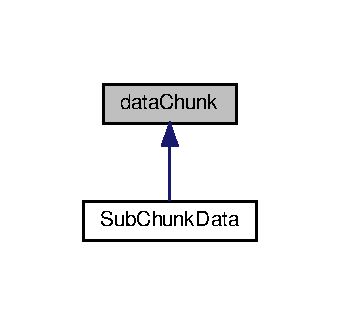
\includegraphics[width=163pt]{structdataChunk__inherit__graph}
\end{center}
\end{figure}
\subsection*{Public Attributes}
\begin{DoxyCompactItemize}
\item 
char \hyperlink{structdataChunk_a846343045c6f7168e969f3a4f19a44e1}{fmt\+\_\+header} \mbox{[}4\mbox{]}
\item 
int \hyperlink{structdataChunk_ab34bbfab5f9c6f68319a493844219a2e}{fmt\+\_\+chunk\+\_\+size}
\end{DoxyCompactItemize}


\subsection{Detailed Description}
This is a data chunk struct 

\subsection{Member Data Documentation}
\mbox{\Hypertarget{structdataChunk_ab34bbfab5f9c6f68319a493844219a2e}\label{structdataChunk_ab34bbfab5f9c6f68319a493844219a2e}} 
\index{data\+Chunk@{data\+Chunk}!fmt\+\_\+chunk\+\_\+size@{fmt\+\_\+chunk\+\_\+size}}
\index{fmt\+\_\+chunk\+\_\+size@{fmt\+\_\+chunk\+\_\+size}!data\+Chunk@{data\+Chunk}}
\subsubsection{\texorpdfstring{fmt\+\_\+chunk\+\_\+size}{fmt\_chunk\_size}}
{\footnotesize\ttfamily int data\+Chunk\+::fmt\+\_\+chunk\+\_\+size}

\mbox{\Hypertarget{structdataChunk_a846343045c6f7168e969f3a4f19a44e1}\label{structdataChunk_a846343045c6f7168e969f3a4f19a44e1}} 
\index{data\+Chunk@{data\+Chunk}!fmt\+\_\+header@{fmt\+\_\+header}}
\index{fmt\+\_\+header@{fmt\+\_\+header}!data\+Chunk@{data\+Chunk}}
\subsubsection{\texorpdfstring{fmt\+\_\+header}{fmt\_header}}
{\footnotesize\ttfamily char data\+Chunk\+::fmt\+\_\+header\mbox{[}4\mbox{]}}



The documentation for this struct was generated from the following file\+:\begin{DoxyCompactItemize}
\item 
\hyperlink{wavHeader_8h}{wav\+Header.\+h}\end{DoxyCompactItemize}

\hypertarget{classEcho}{}\section{Echo Class Reference}
\label{classEcho}\index{Echo@{Echo}}


{\ttfamily \#include $<$echo.\+h$>$}



Inheritance diagram for Echo\+:\nopagebreak
\begin{figure}[H]
\begin{center}
\leavevmode
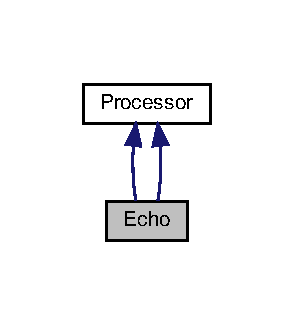
\includegraphics[width=141pt]{classEcho__inherit__graph}
\end{center}
\end{figure}


Collaboration diagram for Echo\+:\nopagebreak
\begin{figure}[H]
\begin{center}
\leavevmode
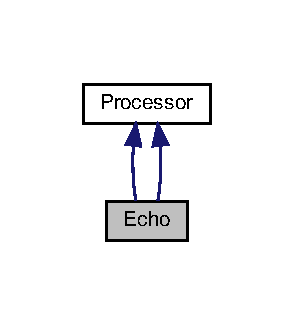
\includegraphics[width=141pt]{classEcho__coll__graph}
\end{center}
\end{figure}
\subsection*{Public Member Functions}
\begin{DoxyCompactItemize}
\item 
\hyperlink{classEcho_ababd42898feed0775f5234d53fe9bff1}{Echo} ()
\item 
\hyperlink{classEcho_a28d71de619dda9e6e51567a04bfb60d6}{Echo} (int new\+Delay)
\item 
int \hyperlink{classEcho_a57e19c9232f9bb96ccd78ba4bb68d6c9}{get\+Delay} ()
\item 
void \hyperlink{classEcho_a3096c57223d6f7ce3097d15e8bf4a0ed}{set\+Delay} (int new\+Delay)
\item 
void \hyperlink{classEcho_a472cc906604bcb493c6a6c1227436938}{processor\+MonoE} (int size, unsigned char $\ast$buffer)
\item 
void \hyperlink{classEcho_a92aa2d47f32f5ad0f2cd45121e8d457f}{processor\+StereoE} (int sizeR, int sizeL, unsigned char $\ast$bufferR, unsigned char $\ast$bufferL)
\item 
void \hyperlink{classEcho_a298f9fe12295c578737928544c46be1a}{processor\+MonoS} (int size, short $\ast$buffer)
\item 
void \hyperlink{classEcho_a26ebcc62f7d6be2e3bd4ac1833636549}{processor\+StereoS} (int sizeR, int sizeL, short $\ast$bufferR, short $\ast$bufferL)
\end{DoxyCompactItemize}


\subsection{Detailed Description}
This is an \hyperlink{classEcho}{Echo} class 

\subsection{Constructor \& Destructor Documentation}
\mbox{\Hypertarget{classEcho_ababd42898feed0775f5234d53fe9bff1}\label{classEcho_ababd42898feed0775f5234d53fe9bff1}} 
\index{Echo@{Echo}!Echo@{Echo}}
\index{Echo@{Echo}!Echo@{Echo}}
\subsubsection{\texorpdfstring{Echo()}{Echo()}\hspace{0.1cm}{\footnotesize\ttfamily [1/2]}}
{\footnotesize\ttfamily Echo\+::\+Echo (\begin{DoxyParamCaption}{ }\end{DoxyParamCaption})}

Base Constructor that takes in the delay for the echo \mbox{\Hypertarget{classEcho_a28d71de619dda9e6e51567a04bfb60d6}\label{classEcho_a28d71de619dda9e6e51567a04bfb60d6}} 
\index{Echo@{Echo}!Echo@{Echo}}
\index{Echo@{Echo}!Echo@{Echo}}
\subsubsection{\texorpdfstring{Echo()}{Echo()}\hspace{0.1cm}{\footnotesize\ttfamily [2/2]}}
{\footnotesize\ttfamily Echo\+::\+Echo (\begin{DoxyParamCaption}\item[{int}]{new\+Delay }\end{DoxyParamCaption})}

Constructor that takes in the delay for the echo 
\begin{DoxyParams}{Parameters}
{\em new\+Delay} & \\
\hline
\end{DoxyParams}


\subsection{Member Function Documentation}
\mbox{\Hypertarget{classEcho_a57e19c9232f9bb96ccd78ba4bb68d6c9}\label{classEcho_a57e19c9232f9bb96ccd78ba4bb68d6c9}} 
\index{Echo@{Echo}!get\+Delay@{get\+Delay}}
\index{get\+Delay@{get\+Delay}!Echo@{Echo}}
\subsubsection{\texorpdfstring{get\+Delay()}{getDelay()}}
{\footnotesize\ttfamily int Echo\+::get\+Delay (\begin{DoxyParamCaption}{ }\end{DoxyParamCaption})}

Getter of delay value \mbox{\Hypertarget{classEcho_a472cc906604bcb493c6a6c1227436938}\label{classEcho_a472cc906604bcb493c6a6c1227436938}} 
\index{Echo@{Echo}!processor\+MonoE@{processor\+MonoE}}
\index{processor\+MonoE@{processor\+MonoE}!Echo@{Echo}}
\subsubsection{\texorpdfstring{processor\+Mono\+E()}{processorMonoE()}}
{\footnotesize\ttfamily void Echo\+::processor\+MonoE (\begin{DoxyParamCaption}\item[{int}]{size,  }\item[{unsigned char $\ast$}]{buffer }\end{DoxyParamCaption})\hspace{0.3cm}{\ttfamily [virtual]}}

Audio \hyperlink{classProcessor}{Processor} for Mono E 
\begin{DoxyParams}{Parameters}
{\em size} & -\/ gets size data \\
\hline
{\em buffer} & -\/ gets range for data \\
\hline
\end{DoxyParams}


Implements \hyperlink{classProcessor_aa9742b5df48a3c6442d521ce93012fc1}{Processor}.

\mbox{\Hypertarget{classEcho_a298f9fe12295c578737928544c46be1a}\label{classEcho_a298f9fe12295c578737928544c46be1a}} 
\index{Echo@{Echo}!processor\+MonoS@{processor\+MonoS}}
\index{processor\+MonoS@{processor\+MonoS}!Echo@{Echo}}
\subsubsection{\texorpdfstring{processor\+Mono\+S()}{processorMonoS()}}
{\footnotesize\ttfamily void Echo\+::processor\+MonoS (\begin{DoxyParamCaption}\item[{int}]{size,  }\item[{short $\ast$}]{buffer }\end{DoxyParamCaption})\hspace{0.3cm}{\ttfamily [virtual]}}

Audio \hyperlink{classProcessor}{Processor} for Mono S 
\begin{DoxyParams}{Parameters}
{\em size} & -\/ gets size data \\
\hline
{\em buffer} & -\/ short integer for buffer \\
\hline
\end{DoxyParams}


Implements \hyperlink{classProcessor_a4cf32c9f7e26383490e8fb49defcc287}{Processor}.

\mbox{\Hypertarget{classEcho_a92aa2d47f32f5ad0f2cd45121e8d457f}\label{classEcho_a92aa2d47f32f5ad0f2cd45121e8d457f}} 
\index{Echo@{Echo}!processor\+StereoE@{processor\+StereoE}}
\index{processor\+StereoE@{processor\+StereoE}!Echo@{Echo}}
\subsubsection{\texorpdfstring{processor\+Stereo\+E()}{processorStereoE()}}
{\footnotesize\ttfamily void Echo\+::processor\+StereoE (\begin{DoxyParamCaption}\item[{int}]{sizeR,  }\item[{int}]{sizeL,  }\item[{unsigned char $\ast$}]{bufferR,  }\item[{unsigned char $\ast$}]{bufferL }\end{DoxyParamCaption})\hspace{0.3cm}{\ttfamily [virtual]}}

Audio \hyperlink{classProcessor}{Processor} for Stereo E 
\begin{DoxyParams}{Parameters}
{\em sizeR} & -\/ gets size data for right side \\
\hline
{\em bufferR} & -\/ gets range for data for right side \\
\hline
{\em bufferL} & -\/ gets range for data for left side \\
\hline
{\em sizeL} & -\/ gets size data for left side \\
\hline
\end{DoxyParams}


Implements \hyperlink{classProcessor_a637904e06d0a3b14f9e1e90fe7f3afbd}{Processor}.

\mbox{\Hypertarget{classEcho_a26ebcc62f7d6be2e3bd4ac1833636549}\label{classEcho_a26ebcc62f7d6be2e3bd4ac1833636549}} 
\index{Echo@{Echo}!processor\+StereoS@{processor\+StereoS}}
\index{processor\+StereoS@{processor\+StereoS}!Echo@{Echo}}
\subsubsection{\texorpdfstring{processor\+Stereo\+S()}{processorStereoS()}}
{\footnotesize\ttfamily void Echo\+::processor\+StereoS (\begin{DoxyParamCaption}\item[{int}]{sizeR,  }\item[{int}]{sizeL,  }\item[{short $\ast$}]{bufferR,  }\item[{short $\ast$}]{bufferL }\end{DoxyParamCaption})\hspace{0.3cm}{\ttfamily [virtual]}}

Audio \hyperlink{classProcessor}{Processor} for Stereo E 
\begin{DoxyParams}{Parameters}
{\em sizeR} & -\/ gets size data for right side \\
\hline
{\em bufferR} & -\/ short integer for buffer on right side \\
\hline
{\em bufferL} & -\/ short integer for buffer on left side \\
\hline
{\em sizeL} & -\/ gets size data for left side \\
\hline
\end{DoxyParams}


Implements \hyperlink{classProcessor_ae3fc266daadbedfa947e596d3ff98a7c}{Processor}.

\mbox{\Hypertarget{classEcho_a3096c57223d6f7ce3097d15e8bf4a0ed}\label{classEcho_a3096c57223d6f7ce3097d15e8bf4a0ed}} 
\index{Echo@{Echo}!set\+Delay@{set\+Delay}}
\index{set\+Delay@{set\+Delay}!Echo@{Echo}}
\subsubsection{\texorpdfstring{set\+Delay()}{setDelay()}}
{\footnotesize\ttfamily void Echo\+::set\+Delay (\begin{DoxyParamCaption}\item[{int}]{new\+Delay }\end{DoxyParamCaption})}

Setter of delay value 
\begin{DoxyParams}{Parameters}
{\em new\+Delay} & \\
\hline
\end{DoxyParams}


The documentation for this class was generated from the following files\+:\begin{DoxyCompactItemize}
\item 
\hyperlink{echo_8h}{echo.\+h}\item 
\hyperlink{echo_8cpp}{echo.\+cpp}\end{DoxyCompactItemize}

\hypertarget{structFMT}{}\section{F\+MT Struct Reference}
\label{structFMT}\index{F\+MT@{F\+MT}}


{\ttfamily \#include $<$wav\+Header.\+h$>$}

\subsection*{Public Attributes}
\begin{DoxyCompactItemize}
\item 
unsigned short \hyperlink{structFMT_a48bb016d6a5a04fb21e5fa5381117d61}{audio\+\_\+format}
\item 
unsigned short \hyperlink{structFMT_a28919c7db5b63cb70af4dc7f8405599e}{num\+\_\+channels}
\item 
int \hyperlink{structFMT_ad09f55ae3078ca9c3545204c4b241910}{sample\+\_\+rate}
\item 
int \hyperlink{structFMT_ada872d0d97744d55e35530140ac22003}{byte\+\_\+rate}
\item 
unsigned short \hyperlink{structFMT_a59c3f8f2f14ff86b8d10cfbf822f71e9}{sample\+\_\+alignment}
\item 
unsigned short \hyperlink{structFMT_a79e51e1ecd1fbb1de975ea73d07e3193}{bit\+\_\+depth}
\end{DoxyCompactItemize}


\subsection{Detailed Description}
This is a \hyperlink{structFMT}{F\+MT} struct 

\subsection{Member Data Documentation}
\mbox{\Hypertarget{structFMT_a48bb016d6a5a04fb21e5fa5381117d61}\label{structFMT_a48bb016d6a5a04fb21e5fa5381117d61}} 
\index{F\+MT@{F\+MT}!audio\+\_\+format@{audio\+\_\+format}}
\index{audio\+\_\+format@{audio\+\_\+format}!F\+MT@{F\+MT}}
\subsubsection{\texorpdfstring{audio\+\_\+format}{audio\_format}}
{\footnotesize\ttfamily unsigned short F\+M\+T\+::audio\+\_\+format}

\mbox{\Hypertarget{structFMT_a79e51e1ecd1fbb1de975ea73d07e3193}\label{structFMT_a79e51e1ecd1fbb1de975ea73d07e3193}} 
\index{F\+MT@{F\+MT}!bit\+\_\+depth@{bit\+\_\+depth}}
\index{bit\+\_\+depth@{bit\+\_\+depth}!F\+MT@{F\+MT}}
\subsubsection{\texorpdfstring{bit\+\_\+depth}{bit\_depth}}
{\footnotesize\ttfamily unsigned short F\+M\+T\+::bit\+\_\+depth}

\mbox{\Hypertarget{structFMT_ada872d0d97744d55e35530140ac22003}\label{structFMT_ada872d0d97744d55e35530140ac22003}} 
\index{F\+MT@{F\+MT}!byte\+\_\+rate@{byte\+\_\+rate}}
\index{byte\+\_\+rate@{byte\+\_\+rate}!F\+MT@{F\+MT}}
\subsubsection{\texorpdfstring{byte\+\_\+rate}{byte\_rate}}
{\footnotesize\ttfamily int F\+M\+T\+::byte\+\_\+rate}

\mbox{\Hypertarget{structFMT_a28919c7db5b63cb70af4dc7f8405599e}\label{structFMT_a28919c7db5b63cb70af4dc7f8405599e}} 
\index{F\+MT@{F\+MT}!num\+\_\+channels@{num\+\_\+channels}}
\index{num\+\_\+channels@{num\+\_\+channels}!F\+MT@{F\+MT}}
\subsubsection{\texorpdfstring{num\+\_\+channels}{num\_channels}}
{\footnotesize\ttfamily unsigned short F\+M\+T\+::num\+\_\+channels}

\mbox{\Hypertarget{structFMT_a59c3f8f2f14ff86b8d10cfbf822f71e9}\label{structFMT_a59c3f8f2f14ff86b8d10cfbf822f71e9}} 
\index{F\+MT@{F\+MT}!sample\+\_\+alignment@{sample\+\_\+alignment}}
\index{sample\+\_\+alignment@{sample\+\_\+alignment}!F\+MT@{F\+MT}}
\subsubsection{\texorpdfstring{sample\+\_\+alignment}{sample\_alignment}}
{\footnotesize\ttfamily unsigned short F\+M\+T\+::sample\+\_\+alignment}

\mbox{\Hypertarget{structFMT_ad09f55ae3078ca9c3545204c4b241910}\label{structFMT_ad09f55ae3078ca9c3545204c4b241910}} 
\index{F\+MT@{F\+MT}!sample\+\_\+rate@{sample\+\_\+rate}}
\index{sample\+\_\+rate@{sample\+\_\+rate}!F\+MT@{F\+MT}}
\subsubsection{\texorpdfstring{sample\+\_\+rate}{sample\_rate}}
{\footnotesize\ttfamily int F\+M\+T\+::sample\+\_\+rate}



The documentation for this struct was generated from the following file\+:\begin{DoxyCompactItemize}
\item 
\hyperlink{wavHeader_8h}{wav\+Header.\+h}\end{DoxyCompactItemize}

\hypertarget{classMdManager}{}\section{Md\+Manager Class Reference}
\label{classMdManager}\index{Md\+Manager@{Md\+Manager}}


{\ttfamily \#include $<$meta\+Data\+Manager.\+h$>$}

\subsection*{Public Member Functions}
\begin{DoxyCompactItemize}
\item 
\hyperlink{classMdManager_a540aeeb85ad958cfbf074316c44d874d}{Md\+Manager} ()=default
\item 
\hyperlink{classMdManager_a9a04c96ea303f2e8d18275ba75af2551}{Md\+Manager} (std\+::ifstream \&)
\item 
void \hyperlink{classMdManager_af9a631c2934e89728ae34be82f78e7fe}{print\+Md} ()
\item 
int \hyperlink{classMdManager_a45e38a55df629208bb6727e10de5ca2c}{get\+Size} () const
\end{DoxyCompactItemize}


\subsection{Detailed Description}
This is an \hyperlink{classMetaData}{Meta\+Data} Manager class 

\subsection{Constructor \& Destructor Documentation}
\mbox{\Hypertarget{classMdManager_a540aeeb85ad958cfbf074316c44d874d}\label{classMdManager_a540aeeb85ad958cfbf074316c44d874d}} 
\index{Md\+Manager@{Md\+Manager}!Md\+Manager@{Md\+Manager}}
\index{Md\+Manager@{Md\+Manager}!Md\+Manager@{Md\+Manager}}
\subsubsection{\texorpdfstring{Md\+Manager()}{MdManager()}\hspace{0.1cm}{\footnotesize\ttfamily [1/2]}}
{\footnotesize\ttfamily Md\+Manager\+::\+Md\+Manager (\begin{DoxyParamCaption}{ }\end{DoxyParamCaption})\hspace{0.3cm}{\ttfamily [default]}}

This is the base constructor \mbox{\Hypertarget{classMdManager_a9a04c96ea303f2e8d18275ba75af2551}\label{classMdManager_a9a04c96ea303f2e8d18275ba75af2551}} 
\index{Md\+Manager@{Md\+Manager}!Md\+Manager@{Md\+Manager}}
\index{Md\+Manager@{Md\+Manager}!Md\+Manager@{Md\+Manager}}
\subsubsection{\texorpdfstring{Md\+Manager()}{MdManager()}\hspace{0.1cm}{\footnotesize\ttfamily [2/2]}}
{\footnotesize\ttfamily Md\+Manager\+::\+Md\+Manager (\begin{DoxyParamCaption}\item[{std\+::ifstream \&}]{file }\end{DoxyParamCaption})}

This contructor calls in the address of the data point 
\begin{DoxyParams}{Parameters}
{\em file} & -\/ address of the data \\
\hline
\end{DoxyParams}


\subsection{Member Function Documentation}
\mbox{\Hypertarget{classMdManager_a45e38a55df629208bb6727e10de5ca2c}\label{classMdManager_a45e38a55df629208bb6727e10de5ca2c}} 
\index{Md\+Manager@{Md\+Manager}!get\+Size@{get\+Size}}
\index{get\+Size@{get\+Size}!Md\+Manager@{Md\+Manager}}
\subsubsection{\texorpdfstring{get\+Size()}{getSize()}}
{\footnotesize\ttfamily int Md\+Manager\+::get\+Size (\begin{DoxyParamCaption}{ }\end{DoxyParamCaption}) const}

This function gets the size of the data (constant) \mbox{\Hypertarget{classMdManager_af9a631c2934e89728ae34be82f78e7fe}\label{classMdManager_af9a631c2934e89728ae34be82f78e7fe}} 
\index{Md\+Manager@{Md\+Manager}!print\+Md@{print\+Md}}
\index{print\+Md@{print\+Md}!Md\+Manager@{Md\+Manager}}
\subsubsection{\texorpdfstring{print\+Md()}{printMd()}}
{\footnotesize\ttfamily void Md\+Manager\+::print\+Md (\begin{DoxyParamCaption}{ }\end{DoxyParamCaption})}

This function prints the metadata 

The documentation for this class was generated from the following files\+:\begin{DoxyCompactItemize}
\item 
\hyperlink{metaDataManager_8h}{meta\+Data\+Manager.\+h}\item 
\hyperlink{metaDataManager_8cpp}{meta\+Data\+Manager.\+cpp}\end{DoxyCompactItemize}

\hypertarget{classmenu}{}\section{menu$<$ T $>$ Class Template Reference}
\label{classmenu}\index{menu$<$ T $>$@{menu$<$ T $>$}}


{\ttfamily \#include $<$menu.\+h$>$}

\subsection*{Public Member Functions}
\begin{DoxyCompactItemize}
\item 
\hyperlink{classmenu_af1685203f74243e56f880ae06443b12a}{menu} ()
\item 
\hyperlink{classmenu_a1ba608803dbd7d3eb5d5f0c7dd58a9f3}{menu} (T user\+Choice)
\item 
T \hyperlink{classmenu_a5ee13e54600aaa2a1202264a2992a493}{switch\+State} ()
\end{DoxyCompactItemize}


\subsection{Detailed Description}
\subsubsection*{template$<$typename T$>$\newline
class menu$<$ T $>$}

This is a Menu class 

\subsection{Constructor \& Destructor Documentation}
\mbox{\Hypertarget{classmenu_af1685203f74243e56f880ae06443b12a}\label{classmenu_af1685203f74243e56f880ae06443b12a}} 
\index{menu@{menu}!menu@{menu}}
\index{menu@{menu}!menu@{menu}}
\subsubsection{\texorpdfstring{menu()}{menu()}\hspace{0.1cm}{\footnotesize\ttfamily [1/2]}}
{\footnotesize\ttfamily template$<$typename T $>$ \\
\hyperlink{classmenu}{menu}$<$ T $>$\+::\hyperlink{classmenu}{menu} (\begin{DoxyParamCaption}{ }\end{DoxyParamCaption})}

Base Constructor \mbox{\Hypertarget{classmenu_a1ba608803dbd7d3eb5d5f0c7dd58a9f3}\label{classmenu_a1ba608803dbd7d3eb5d5f0c7dd58a9f3}} 
\index{menu@{menu}!menu@{menu}}
\index{menu@{menu}!menu@{menu}}
\subsubsection{\texorpdfstring{menu()}{menu()}\hspace{0.1cm}{\footnotesize\ttfamily [2/2]}}
{\footnotesize\ttfamily template$<$typename T $>$ \\
\hyperlink{classmenu}{menu}$<$ T $>$\+::\hyperlink{classmenu}{menu} (\begin{DoxyParamCaption}\item[{T}]{user\+Choice }\end{DoxyParamCaption})}

Constructor that takes in the use\+Choice template 
\begin{DoxyParams}{Parameters}
{\em user\+Choice} & -\/ Template for users to choose options \\
\hline
\end{DoxyParams}


\subsection{Member Function Documentation}
\mbox{\Hypertarget{classmenu_a5ee13e54600aaa2a1202264a2992a493}\label{classmenu_a5ee13e54600aaa2a1202264a2992a493}} 
\index{menu@{menu}!switch\+State@{switch\+State}}
\index{switch\+State@{switch\+State}!menu@{menu}}
\subsubsection{\texorpdfstring{switch\+State()}{switchState()}}
{\footnotesize\ttfamily template$<$typename T $>$ \\
T \hyperlink{classmenu}{menu}$<$ T $>$\+::switch\+State (\begin{DoxyParamCaption}{ }\end{DoxyParamCaption})}

This is our template T using switch cases for the user interface Here is the caller graph for this function\+:\nopagebreak
\begin{figure}[H]
\begin{center}
\leavevmode
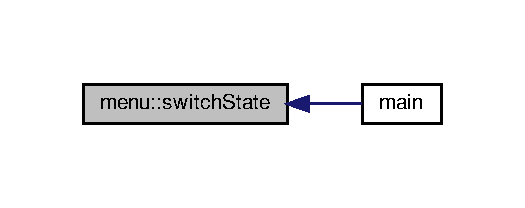
\includegraphics[width=252pt]{classmenu_a5ee13e54600aaa2a1202264a2992a493_icgraph}
\end{center}
\end{figure}


The documentation for this class was generated from the following file\+:\begin{DoxyCompactItemize}
\item 
\hyperlink{menu_8h}{menu.\+h}\end{DoxyCompactItemize}

\hypertarget{classMetaData}{}\section{Meta\+Data Class Reference}
\label{classMetaData}\index{Meta\+Data@{Meta\+Data}}


{\ttfamily \#include $<$meta\+Data.\+h$>$}

\subsection*{Public Member Functions}
\begin{DoxyCompactItemize}
\item 
\hyperlink{classMetaData_a666d1eea92f7243c39dae95de0352b11}{Meta\+Data} ()=default
\item 
\hyperlink{classMetaData_aac49325e3507e976fb41690bfa6be536}{Meta\+Data} (std\+::ifstream \&)
\item 
std\+::string \hyperlink{classMetaData_ad46cdaa2d7d988b9f73cd3c438dd9cb9}{get\+Md\+ID} () const
\item 
void \hyperlink{classMetaData_ad16be865033e4856cf1eaab2dd6e5409}{set\+Md\+ID} (char) const
\item 
int \hyperlink{classMetaData_ab013c35f16c09bc6e69164c2c6df5b46}{get\+Md\+Size} () const
\item 
void \hyperlink{classMetaData_aa500b5bcfc28dfc1f0b32b7fcdca108f}{set\+Md\+Size} (int)
\item 
std\+::string \hyperlink{classMetaData_a105bbcd8cfee4f70c0942ec67154079a}{get\+Buffer} () const
\item 
void \hyperlink{classMetaData_a8993ecf3ca590b956fd1c7383a3f5c24}{set\+Buffer} (std\+::string)
\end{DoxyCompactItemize}


\subsection{Detailed Description}
This is an \hyperlink{classMetaData}{Meta\+Data} class 

\subsection{Constructor \& Destructor Documentation}
\mbox{\Hypertarget{classMetaData_a666d1eea92f7243c39dae95de0352b11}\label{classMetaData_a666d1eea92f7243c39dae95de0352b11}} 
\index{Meta\+Data@{Meta\+Data}!Meta\+Data@{Meta\+Data}}
\index{Meta\+Data@{Meta\+Data}!Meta\+Data@{Meta\+Data}}
\subsubsection{\texorpdfstring{Meta\+Data()}{MetaData()}\hspace{0.1cm}{\footnotesize\ttfamily [1/2]}}
{\footnotesize\ttfamily Meta\+Data\+::\+Meta\+Data (\begin{DoxyParamCaption}{ }\end{DoxyParamCaption})\hspace{0.3cm}{\ttfamily [default]}}

This is the base constructor \mbox{\Hypertarget{classMetaData_aac49325e3507e976fb41690bfa6be536}\label{classMetaData_aac49325e3507e976fb41690bfa6be536}} 
\index{Meta\+Data@{Meta\+Data}!Meta\+Data@{Meta\+Data}}
\index{Meta\+Data@{Meta\+Data}!Meta\+Data@{Meta\+Data}}
\subsubsection{\texorpdfstring{Meta\+Data()}{MetaData()}\hspace{0.1cm}{\footnotesize\ttfamily [2/2]}}
{\footnotesize\ttfamily Meta\+Data\+::\+Meta\+Data (\begin{DoxyParamCaption}\item[{std\+::ifstream \&}]{file }\end{DoxyParamCaption})}

Constructor that is responsible for reading the metadata 
\begin{DoxyParams}{Parameters}
{\em file} & -\/ address of the data \\
\hline
\end{DoxyParams}
Here is the call graph for this function\+:\nopagebreak
\begin{figure}[H]
\begin{center}
\leavevmode
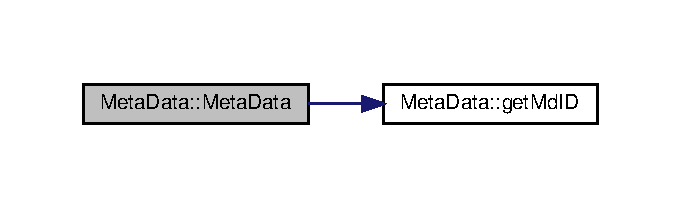
\includegraphics[width=327pt]{classMetaData_aac49325e3507e976fb41690bfa6be536_cgraph}
\end{center}
\end{figure}


\subsection{Member Function Documentation}
\mbox{\Hypertarget{classMetaData_a105bbcd8cfee4f70c0942ec67154079a}\label{classMetaData_a105bbcd8cfee4f70c0942ec67154079a}} 
\index{Meta\+Data@{Meta\+Data}!get\+Buffer@{get\+Buffer}}
\index{get\+Buffer@{get\+Buffer}!Meta\+Data@{Meta\+Data}}
\subsubsection{\texorpdfstring{get\+Buffer()}{getBuffer()}}
{\footnotesize\ttfamily std\+::string Meta\+Data\+::get\+Buffer (\begin{DoxyParamCaption}{ }\end{DoxyParamCaption}) const}

Getter of buffer \mbox{\Hypertarget{classMetaData_ad46cdaa2d7d988b9f73cd3c438dd9cb9}\label{classMetaData_ad46cdaa2d7d988b9f73cd3c438dd9cb9}} 
\index{Meta\+Data@{Meta\+Data}!get\+Md\+ID@{get\+Md\+ID}}
\index{get\+Md\+ID@{get\+Md\+ID}!Meta\+Data@{Meta\+Data}}
\subsubsection{\texorpdfstring{get\+Md\+I\+D()}{getMdID()}}
{\footnotesize\ttfamily std\+::string Meta\+Data\+::get\+Md\+ID (\begin{DoxyParamCaption}{ }\end{DoxyParamCaption}) const}

Getter of metadata ID Here is the caller graph for this function\+:\nopagebreak
\begin{figure}[H]
\begin{center}
\leavevmode
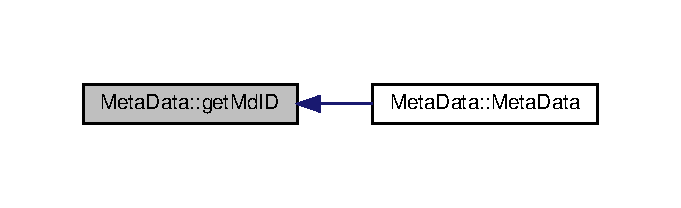
\includegraphics[width=327pt]{classMetaData_ad46cdaa2d7d988b9f73cd3c438dd9cb9_icgraph}
\end{center}
\end{figure}
\mbox{\Hypertarget{classMetaData_ab013c35f16c09bc6e69164c2c6df5b46}\label{classMetaData_ab013c35f16c09bc6e69164c2c6df5b46}} 
\index{Meta\+Data@{Meta\+Data}!get\+Md\+Size@{get\+Md\+Size}}
\index{get\+Md\+Size@{get\+Md\+Size}!Meta\+Data@{Meta\+Data}}
\subsubsection{\texorpdfstring{get\+Md\+Size()}{getMdSize()}}
{\footnotesize\ttfamily int Meta\+Data\+::get\+Md\+Size (\begin{DoxyParamCaption}{ }\end{DoxyParamCaption}) const}

Getter of metadata size \mbox{\Hypertarget{classMetaData_a8993ecf3ca590b956fd1c7383a3f5c24}\label{classMetaData_a8993ecf3ca590b956fd1c7383a3f5c24}} 
\index{Meta\+Data@{Meta\+Data}!set\+Buffer@{set\+Buffer}}
\index{set\+Buffer@{set\+Buffer}!Meta\+Data@{Meta\+Data}}
\subsubsection{\texorpdfstring{set\+Buffer()}{setBuffer()}}
{\footnotesize\ttfamily void Meta\+Data\+::set\+Buffer (\begin{DoxyParamCaption}\item[{std\+::string}]{buffer }\end{DoxyParamCaption})}

Setter of buffer Returns a string \mbox{\Hypertarget{classMetaData_ad16be865033e4856cf1eaab2dd6e5409}\label{classMetaData_ad16be865033e4856cf1eaab2dd6e5409}} 
\index{Meta\+Data@{Meta\+Data}!set\+Md\+ID@{set\+Md\+ID}}
\index{set\+Md\+ID@{set\+Md\+ID}!Meta\+Data@{Meta\+Data}}
\subsubsection{\texorpdfstring{set\+Md\+I\+D()}{setMdID()}}
{\footnotesize\ttfamily void Meta\+Data\+::set\+Md\+ID (\begin{DoxyParamCaption}\item[{char}]{ }\end{DoxyParamCaption}) const}

Setter of metadata ID Returns a constant char \mbox{\Hypertarget{classMetaData_aa500b5bcfc28dfc1f0b32b7fcdca108f}\label{classMetaData_aa500b5bcfc28dfc1f0b32b7fcdca108f}} 
\index{Meta\+Data@{Meta\+Data}!set\+Md\+Size@{set\+Md\+Size}}
\index{set\+Md\+Size@{set\+Md\+Size}!Meta\+Data@{Meta\+Data}}
\subsubsection{\texorpdfstring{set\+Md\+Size()}{setMdSize()}}
{\footnotesize\ttfamily void Meta\+Data\+::set\+Md\+Size (\begin{DoxyParamCaption}\item[{int}]{md\+Size }\end{DoxyParamCaption})}

Setter of metadata ID Returns a integer 

The documentation for this class was generated from the following files\+:\begin{DoxyCompactItemize}
\item 
\hyperlink{metaData_8h}{meta\+Data.\+h}\item 
\hyperlink{metaData_8cpp}{meta\+Data.\+cpp}\end{DoxyCompactItemize}

\hypertarget{structMetaDataHeader}{}\section{Meta\+Data\+Header Struct Reference}
\label{structMetaDataHeader}\index{Meta\+Data\+Header@{Meta\+Data\+Header}}


{\ttfamily \#include $<$meta\+Data\+Header.\+h$>$}

\subsection*{Public Attributes}
\begin{DoxyCompactItemize}
\item 
char \hyperlink{structMetaDataHeader_af7f56239f7f1b01f7f6ae8add64205ed}{list\+\_\+\+ID} \mbox{[}4\mbox{]}
\item 
int \hyperlink{structMetaDataHeader_aa235aaa4faacbabeefff7826c26138aa}{list\+\_\+size}
\item 
char \hyperlink{structMetaDataHeader_a779d334b540619b63dca0e358541a090}{info\+\_\+\+ID} \mbox{[}4\mbox{]}
\end{DoxyCompactItemize}


\subsection{Detailed Description}
This is an \hyperlink{structMetaDataHeader}{Meta\+Data\+Header} struct 

\subsection{Member Data Documentation}
\mbox{\Hypertarget{structMetaDataHeader_a779d334b540619b63dca0e358541a090}\label{structMetaDataHeader_a779d334b540619b63dca0e358541a090}} 
\index{Meta\+Data\+Header@{Meta\+Data\+Header}!info\+\_\+\+ID@{info\+\_\+\+ID}}
\index{info\+\_\+\+ID@{info\+\_\+\+ID}!Meta\+Data\+Header@{Meta\+Data\+Header}}
\subsubsection{\texorpdfstring{info\+\_\+\+ID}{info\_ID}}
{\footnotesize\ttfamily char Meta\+Data\+Header\+::info\+\_\+\+ID\mbox{[}4\mbox{]}}

\mbox{\Hypertarget{structMetaDataHeader_af7f56239f7f1b01f7f6ae8add64205ed}\label{structMetaDataHeader_af7f56239f7f1b01f7f6ae8add64205ed}} 
\index{Meta\+Data\+Header@{Meta\+Data\+Header}!list\+\_\+\+ID@{list\+\_\+\+ID}}
\index{list\+\_\+\+ID@{list\+\_\+\+ID}!Meta\+Data\+Header@{Meta\+Data\+Header}}
\subsubsection{\texorpdfstring{list\+\_\+\+ID}{list\_ID}}
{\footnotesize\ttfamily char Meta\+Data\+Header\+::list\+\_\+\+ID\mbox{[}4\mbox{]}}

\mbox{\Hypertarget{structMetaDataHeader_aa235aaa4faacbabeefff7826c26138aa}\label{structMetaDataHeader_aa235aaa4faacbabeefff7826c26138aa}} 
\index{Meta\+Data\+Header@{Meta\+Data\+Header}!list\+\_\+size@{list\+\_\+size}}
\index{list\+\_\+size@{list\+\_\+size}!Meta\+Data\+Header@{Meta\+Data\+Header}}
\subsubsection{\texorpdfstring{list\+\_\+size}{list\_size}}
{\footnotesize\ttfamily int Meta\+Data\+Header\+::list\+\_\+size}



The documentation for this struct was generated from the following file\+:\begin{DoxyCompactItemize}
\item 
\hyperlink{metaDataHeader_8h}{meta\+Data\+Header.\+h}\end{DoxyCompactItemize}

\hypertarget{classNoiseGate}{}\section{Noise\+Gate Class Reference}
\label{classNoiseGate}\index{Noise\+Gate@{Noise\+Gate}}


{\ttfamily \#include $<$noiseg\+\_\+diag.\+h$>$}



Inheritance diagram for Noise\+Gate\+:\nopagebreak
\begin{figure}[H]
\begin{center}
\leavevmode
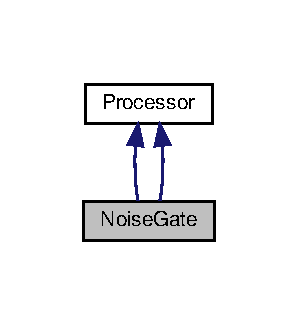
\includegraphics[width=143pt]{classNoiseGate__inherit__graph}
\end{center}
\end{figure}


Collaboration diagram for Noise\+Gate\+:\nopagebreak
\begin{figure}[H]
\begin{center}
\leavevmode
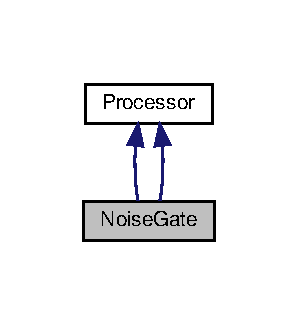
\includegraphics[width=143pt]{classNoiseGate__coll__graph}
\end{center}
\end{figure}
\subsection*{Public Member Functions}
\begin{DoxyCompactItemize}
\item 
\hyperlink{classNoiseGate_ae9ccbe5934108f756ada0e492db5f71e}{Noise\+Gate} ()
\item 
\hyperlink{classNoiseGate_a595f0fbe191ba5eaed8b52c8f2c5049f}{Noise\+Gate} (double level)
\item 
double \hyperlink{classNoiseGate_a48958705ac7b9de4cfe5ae284b8fb4f6}{get\+Level} ()
\item 
void \hyperlink{classNoiseGate_aa03603d23e350f5d9d1e0914de862f57}{set\+Level} (double level)
\item 
void \hyperlink{classNoiseGate_ab2965cbd79e9bb7cd5d972967d3da678}{processor\+MonoE} (int size, unsigned char $\ast$buffer)
\item 
void \hyperlink{classNoiseGate_a3b6bbb8efccac794fe3abf6dbbd92c1f}{processor\+StereoE} (int sizeR, int sizeL, unsigned char $\ast$bufferR, unsigned char $\ast$bufferL)
\item 
void \hyperlink{classNoiseGate_a46b2ad11fa1dac657450c2299026bee4}{processor\+MonoS} (int size, short $\ast$buffer)
\item 
void \hyperlink{classNoiseGate_aa45ac001ec6d3dd7ad935cf92266a285}{processor\+StereoS} (int sizeR, int sizeL, short $\ast$bufferR, short $\ast$bufferL)
\end{DoxyCompactItemize}


\subsection{Detailed Description}
This is a Noise Gate class 

\subsection{Constructor \& Destructor Documentation}
\mbox{\Hypertarget{classNoiseGate_ae9ccbe5934108f756ada0e492db5f71e}\label{classNoiseGate_ae9ccbe5934108f756ada0e492db5f71e}} 
\index{Noise\+Gate@{Noise\+Gate}!Noise\+Gate@{Noise\+Gate}}
\index{Noise\+Gate@{Noise\+Gate}!Noise\+Gate@{Noise\+Gate}}
\subsubsection{\texorpdfstring{Noise\+Gate()}{NoiseGate()}\hspace{0.1cm}{\footnotesize\ttfamily [1/2]}}
{\footnotesize\ttfamily Noise\+Gate\+::\+Noise\+Gate (\begin{DoxyParamCaption}{ }\end{DoxyParamCaption})}

This is the base constructor \mbox{\Hypertarget{classNoiseGate_a595f0fbe191ba5eaed8b52c8f2c5049f}\label{classNoiseGate_a595f0fbe191ba5eaed8b52c8f2c5049f}} 
\index{Noise\+Gate@{Noise\+Gate}!Noise\+Gate@{Noise\+Gate}}
\index{Noise\+Gate@{Noise\+Gate}!Noise\+Gate@{Noise\+Gate}}
\subsubsection{\texorpdfstring{Noise\+Gate()}{NoiseGate()}\hspace{0.1cm}{\footnotesize\ttfamily [2/2]}}
{\footnotesize\ttfamily Noise\+Gate\+::\+Noise\+Gate (\begin{DoxyParamCaption}\item[{double}]{level }\end{DoxyParamCaption})}

This constructor gets the noise gate level 
\begin{DoxyParams}{Parameters}
{\em level} & -\/ level of noise gate as a double data type \\
\hline
\end{DoxyParams}


\subsection{Member Function Documentation}
\mbox{\Hypertarget{classNoiseGate_a48958705ac7b9de4cfe5ae284b8fb4f6}\label{classNoiseGate_a48958705ac7b9de4cfe5ae284b8fb4f6}} 
\index{Noise\+Gate@{Noise\+Gate}!get\+Level@{get\+Level}}
\index{get\+Level@{get\+Level}!Noise\+Gate@{Noise\+Gate}}
\subsubsection{\texorpdfstring{get\+Level()}{getLevel()}}
{\footnotesize\ttfamily double Noise\+Gate\+::get\+Level (\begin{DoxyParamCaption}{ }\end{DoxyParamCaption})}

Getter that gets noise gate level \mbox{\Hypertarget{classNoiseGate_ab2965cbd79e9bb7cd5d972967d3da678}\label{classNoiseGate_ab2965cbd79e9bb7cd5d972967d3da678}} 
\index{Noise\+Gate@{Noise\+Gate}!processor\+MonoE@{processor\+MonoE}}
\index{processor\+MonoE@{processor\+MonoE}!Noise\+Gate@{Noise\+Gate}}
\subsubsection{\texorpdfstring{processor\+Mono\+E()}{processorMonoE()}}
{\footnotesize\ttfamily void Noise\+Gate\+::processor\+MonoE (\begin{DoxyParamCaption}\item[{int}]{size,  }\item[{unsigned char $\ast$}]{buffer }\end{DoxyParamCaption})\hspace{0.3cm}{\ttfamily [virtual]}}

Audio \hyperlink{classProcessor}{Processor} for Mono E 
\begin{DoxyParams}{Parameters}
{\em size} & -\/ gets size data \\
\hline
{\em buffer} & -\/ gets range for data \\
\hline
\end{DoxyParams}


Implements \hyperlink{classProcessor_aa9742b5df48a3c6442d521ce93012fc1}{Processor}.

\mbox{\Hypertarget{classNoiseGate_a46b2ad11fa1dac657450c2299026bee4}\label{classNoiseGate_a46b2ad11fa1dac657450c2299026bee4}} 
\index{Noise\+Gate@{Noise\+Gate}!processor\+MonoS@{processor\+MonoS}}
\index{processor\+MonoS@{processor\+MonoS}!Noise\+Gate@{Noise\+Gate}}
\subsubsection{\texorpdfstring{processor\+Mono\+S()}{processorMonoS()}}
{\footnotesize\ttfamily void Noise\+Gate\+::processor\+MonoS (\begin{DoxyParamCaption}\item[{int}]{size,  }\item[{short $\ast$}]{buffer }\end{DoxyParamCaption})\hspace{0.3cm}{\ttfamily [virtual]}}

Audio \hyperlink{classProcessor}{Processor} for Mono S 
\begin{DoxyParams}{Parameters}
{\em size} & -\/ gets size data \\
\hline
{\em buffer} & -\/ short integer for buffer \\
\hline
\end{DoxyParams}


Implements \hyperlink{classProcessor_a4cf32c9f7e26383490e8fb49defcc287}{Processor}.

\mbox{\Hypertarget{classNoiseGate_a3b6bbb8efccac794fe3abf6dbbd92c1f}\label{classNoiseGate_a3b6bbb8efccac794fe3abf6dbbd92c1f}} 
\index{Noise\+Gate@{Noise\+Gate}!processor\+StereoE@{processor\+StereoE}}
\index{processor\+StereoE@{processor\+StereoE}!Noise\+Gate@{Noise\+Gate}}
\subsubsection{\texorpdfstring{processor\+Stereo\+E()}{processorStereoE()}}
{\footnotesize\ttfamily void Noise\+Gate\+::processor\+StereoE (\begin{DoxyParamCaption}\item[{int}]{sizeR,  }\item[{int}]{sizeL,  }\item[{unsigned char $\ast$}]{bufferR,  }\item[{unsigned char $\ast$}]{bufferL }\end{DoxyParamCaption})\hspace{0.3cm}{\ttfamily [virtual]}}

Audio \hyperlink{classProcessor}{Processor} for Stereo E 
\begin{DoxyParams}{Parameters}
{\em sizeR} & -\/ gets size data for right side \\
\hline
{\em bufferR} & -\/ gets range for data for right side \\
\hline
{\em bufferL} & -\/ gets range for data for left side \\
\hline
{\em sizeL} & -\/ gets size data for left side \\
\hline
\end{DoxyParams}


Implements \hyperlink{classProcessor_a637904e06d0a3b14f9e1e90fe7f3afbd}{Processor}.

\mbox{\Hypertarget{classNoiseGate_aa45ac001ec6d3dd7ad935cf92266a285}\label{classNoiseGate_aa45ac001ec6d3dd7ad935cf92266a285}} 
\index{Noise\+Gate@{Noise\+Gate}!processor\+StereoS@{processor\+StereoS}}
\index{processor\+StereoS@{processor\+StereoS}!Noise\+Gate@{Noise\+Gate}}
\subsubsection{\texorpdfstring{processor\+Stereo\+S()}{processorStereoS()}}
{\footnotesize\ttfamily void Noise\+Gate\+::processor\+StereoS (\begin{DoxyParamCaption}\item[{int}]{sizeR,  }\item[{int}]{sizeL,  }\item[{short $\ast$}]{bufferR,  }\item[{short $\ast$}]{bufferL }\end{DoxyParamCaption})\hspace{0.3cm}{\ttfamily [virtual]}}

Audio \hyperlink{classProcessor}{Processor} for Stereo S 
\begin{DoxyParams}{Parameters}
{\em sizeR} & -\/ gets size data for right side \\
\hline
{\em bufferR} & -\/ short integer for buffer on right side \\
\hline
{\em bufferL} & -\/ short integer for buffer on left side \\
\hline
{\em sizeL} & -\/ gets size data for left side \\
\hline
\end{DoxyParams}


Implements \hyperlink{classProcessor_ae3fc266daadbedfa947e596d3ff98a7c}{Processor}.

\mbox{\Hypertarget{classNoiseGate_aa03603d23e350f5d9d1e0914de862f57}\label{classNoiseGate_aa03603d23e350f5d9d1e0914de862f57}} 
\index{Noise\+Gate@{Noise\+Gate}!set\+Level@{set\+Level}}
\index{set\+Level@{set\+Level}!Noise\+Gate@{Noise\+Gate}}
\subsubsection{\texorpdfstring{set\+Level()}{setLevel()}}
{\footnotesize\ttfamily void Noise\+Gate\+::set\+Level (\begin{DoxyParamCaption}\item[{double}]{level }\end{DoxyParamCaption})}

Setter that gets noise gate level 
\begin{DoxyParams}{Parameters}
{\em level} & -\/ level of noise gate as a double data type \\
\hline
\end{DoxyParams}


The documentation for this class was generated from the following files\+:\begin{DoxyCompactItemize}
\item 
\hyperlink{noiseg__diag_8h}{noiseg\+\_\+diag.\+h}\item 
\hyperlink{noiseGate_8h}{noise\+Gate.\+h}\item 
\hyperlink{noiseGate_8cpp}{noise\+Gate.\+cpp}\end{DoxyCompactItemize}

\hypertarget{classNormalization}{}\section{Normalization Class Reference}
\label{classNormalization}\index{Normalization@{Normalization}}


{\ttfamily \#include $<$norm\+\_\+diag.\+h$>$}



Inheritance diagram for Normalization\+:\nopagebreak
\begin{figure}[H]
\begin{center}
\leavevmode
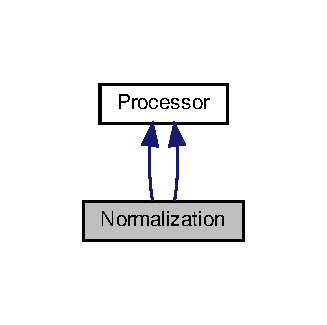
\includegraphics[width=157pt]{classNormalization__inherit__graph}
\end{center}
\end{figure}


Collaboration diagram for Normalization\+:\nopagebreak
\begin{figure}[H]
\begin{center}
\leavevmode
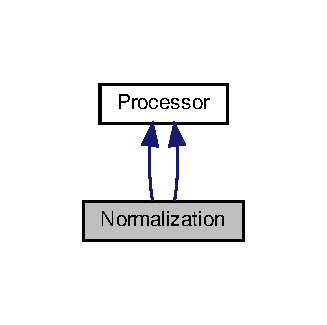
\includegraphics[width=157pt]{classNormalization__coll__graph}
\end{center}
\end{figure}
\subsection*{Public Member Functions}
\begin{DoxyCompactItemize}
\item 
\hyperlink{classNormalization_a7998284e5456d915ebdb2520e4d74250}{Normalization} ()
\item 
\hyperlink{classNormalization_ac4807a0ce2a2d845bd0a8fd0f1fac662}{Normalization} (int new\+Adjust\+Level)
\item 
int \hyperlink{classNormalization_a8e62b273415300146b260ec18561a448}{get\+Adjust\+Level} ()
\item 
void \hyperlink{classNormalization_a4f80ce5334c763075e612688c03edd58}{set\+Adjust\+Level} (int new\+Adjust\+Level)
\item 
void \hyperlink{classNormalization_a61d6afdd8530c60ef098c2e404841683}{processor\+MonoE} (int size, unsigned char $\ast$buffer)
\item 
void \hyperlink{classNormalization_a27a14c9e1a86b55db654335e79c89782}{processor\+StereoE} (int sizeR, int sizeL, unsigned char $\ast$bufferR, unsigned char $\ast$bufferL)
\item 
void \hyperlink{classNormalization_a432fc3b7ef40314bb4d7a215fddc8d0b}{processor\+MonoS} (int size, short $\ast$buffer)
\item 
void \hyperlink{classNormalization_a3221f7132aa5feabc417fbf9ce97e290}{processor\+StereoS} (int sizeR, int sizeL, short $\ast$bufferR, short $\ast$bufferL)
\end{DoxyCompactItemize}


\subsection{Detailed Description}
This is a \hyperlink{classNormalization}{Normalization} class 

\subsection{Constructor \& Destructor Documentation}
\mbox{\Hypertarget{classNormalization_a7998284e5456d915ebdb2520e4d74250}\label{classNormalization_a7998284e5456d915ebdb2520e4d74250}} 
\index{Normalization@{Normalization}!Normalization@{Normalization}}
\index{Normalization@{Normalization}!Normalization@{Normalization}}
\subsubsection{\texorpdfstring{Normalization()}{Normalization()}\hspace{0.1cm}{\footnotesize\ttfamily [1/2]}}
{\footnotesize\ttfamily Normalization\+::\+Normalization (\begin{DoxyParamCaption}{ }\end{DoxyParamCaption})}

Base constructor of normalization \mbox{\Hypertarget{classNormalization_ac4807a0ce2a2d845bd0a8fd0f1fac662}\label{classNormalization_ac4807a0ce2a2d845bd0a8fd0f1fac662}} 
\index{Normalization@{Normalization}!Normalization@{Normalization}}
\index{Normalization@{Normalization}!Normalization@{Normalization}}
\subsubsection{\texorpdfstring{Normalization()}{Normalization()}\hspace{0.1cm}{\footnotesize\ttfamily [2/2]}}
{\footnotesize\ttfamily Normalization\+::\+Normalization (\begin{DoxyParamCaption}\item[{int}]{new\+Adjust\+Level }\end{DoxyParamCaption})}

\hyperlink{classNormalization}{Normalization} constructor for new adjusted level 
\begin{DoxyParams}{Parameters}
{\em new\+Adjusted\+Level} & -\/ takes in the new level after normalization of audio \\
\hline
\end{DoxyParams}


\subsection{Member Function Documentation}
\mbox{\Hypertarget{classNormalization_a8e62b273415300146b260ec18561a448}\label{classNormalization_a8e62b273415300146b260ec18561a448}} 
\index{Normalization@{Normalization}!get\+Adjust\+Level@{get\+Adjust\+Level}}
\index{get\+Adjust\+Level@{get\+Adjust\+Level}!Normalization@{Normalization}}
\subsubsection{\texorpdfstring{get\+Adjust\+Level()}{getAdjustLevel()}}
{\footnotesize\ttfamily int Normalization\+::get\+Adjust\+Level (\begin{DoxyParamCaption}{ }\end{DoxyParamCaption})}

Getter for adjusted level \mbox{\Hypertarget{classNormalization_a61d6afdd8530c60ef098c2e404841683}\label{classNormalization_a61d6afdd8530c60ef098c2e404841683}} 
\index{Normalization@{Normalization}!processor\+MonoE@{processor\+MonoE}}
\index{processor\+MonoE@{processor\+MonoE}!Normalization@{Normalization}}
\subsubsection{\texorpdfstring{processor\+Mono\+E()}{processorMonoE()}}
{\footnotesize\ttfamily void Normalization\+::processor\+MonoE (\begin{DoxyParamCaption}\item[{int}]{size,  }\item[{unsigned char $\ast$}]{buffer }\end{DoxyParamCaption})\hspace{0.3cm}{\ttfamily [virtual]}}

Audio \hyperlink{classProcessor}{Processor} for Mono E 
\begin{DoxyParams}{Parameters}
{\em size} & -\/ gets size data \\
\hline
{\em buffer} & -\/ gets range for data \\
\hline
\end{DoxyParams}


Implements \hyperlink{classProcessor_aa9742b5df48a3c6442d521ce93012fc1}{Processor}.

\mbox{\Hypertarget{classNormalization_a432fc3b7ef40314bb4d7a215fddc8d0b}\label{classNormalization_a432fc3b7ef40314bb4d7a215fddc8d0b}} 
\index{Normalization@{Normalization}!processor\+MonoS@{processor\+MonoS}}
\index{processor\+MonoS@{processor\+MonoS}!Normalization@{Normalization}}
\subsubsection{\texorpdfstring{processor\+Mono\+S()}{processorMonoS()}}
{\footnotesize\ttfamily void Normalization\+::processor\+MonoS (\begin{DoxyParamCaption}\item[{int}]{size,  }\item[{short $\ast$}]{buffer }\end{DoxyParamCaption})\hspace{0.3cm}{\ttfamily [virtual]}}

Audio \hyperlink{classProcessor}{Processor} for Mono S 
\begin{DoxyParams}{Parameters}
{\em size} & -\/ gets size data \\
\hline
{\em buffer} & -\/ short integer for buffer \\
\hline
\end{DoxyParams}


Implements \hyperlink{classProcessor_a4cf32c9f7e26383490e8fb49defcc287}{Processor}.

\mbox{\Hypertarget{classNormalization_a27a14c9e1a86b55db654335e79c89782}\label{classNormalization_a27a14c9e1a86b55db654335e79c89782}} 
\index{Normalization@{Normalization}!processor\+StereoE@{processor\+StereoE}}
\index{processor\+StereoE@{processor\+StereoE}!Normalization@{Normalization}}
\subsubsection{\texorpdfstring{processor\+Stereo\+E()}{processorStereoE()}}
{\footnotesize\ttfamily void Normalization\+::processor\+StereoE (\begin{DoxyParamCaption}\item[{int}]{sizeR,  }\item[{int}]{sizeL,  }\item[{unsigned char $\ast$}]{bufferR,  }\item[{unsigned char $\ast$}]{bufferL }\end{DoxyParamCaption})\hspace{0.3cm}{\ttfamily [virtual]}}

Audio \hyperlink{classProcessor}{Processor} for Stereo E 
\begin{DoxyParams}{Parameters}
{\em sizeR} & -\/ gets size data for right side \\
\hline
{\em bufferR} & -\/ gets range for data for right side \\
\hline
{\em bufferL} & -\/ gets range for data for left side \\
\hline
{\em sizeL} & -\/ gets size data for left side \\
\hline
\end{DoxyParams}


Implements \hyperlink{classProcessor_a637904e06d0a3b14f9e1e90fe7f3afbd}{Processor}.

\mbox{\Hypertarget{classNormalization_a3221f7132aa5feabc417fbf9ce97e290}\label{classNormalization_a3221f7132aa5feabc417fbf9ce97e290}} 
\index{Normalization@{Normalization}!processor\+StereoS@{processor\+StereoS}}
\index{processor\+StereoS@{processor\+StereoS}!Normalization@{Normalization}}
\subsubsection{\texorpdfstring{processor\+Stereo\+S()}{processorStereoS()}}
{\footnotesize\ttfamily void Normalization\+::processor\+StereoS (\begin{DoxyParamCaption}\item[{int}]{sizeR,  }\item[{int}]{sizeL,  }\item[{short $\ast$}]{bufferR,  }\item[{short $\ast$}]{bufferL }\end{DoxyParamCaption})\hspace{0.3cm}{\ttfamily [virtual]}}

Audio \hyperlink{classProcessor}{Processor} for Stereo E 
\begin{DoxyParams}{Parameters}
{\em sizeR} & -\/ gets size data for right side \\
\hline
{\em bufferR} & -\/ short integer for buffer on right side \\
\hline
{\em bufferL} & -\/ short integer for buffer on left side \\
\hline
{\em sizeL} & -\/ gets size data for left side \\
\hline
\end{DoxyParams}


Implements \hyperlink{classProcessor_ae3fc266daadbedfa947e596d3ff98a7c}{Processor}.

\mbox{\Hypertarget{classNormalization_a4f80ce5334c763075e612688c03edd58}\label{classNormalization_a4f80ce5334c763075e612688c03edd58}} 
\index{Normalization@{Normalization}!set\+Adjust\+Level@{set\+Adjust\+Level}}
\index{set\+Adjust\+Level@{set\+Adjust\+Level}!Normalization@{Normalization}}
\subsubsection{\texorpdfstring{set\+Adjust\+Level()}{setAdjustLevel()}}
{\footnotesize\ttfamily void Normalization\+::set\+Adjust\+Level (\begin{DoxyParamCaption}\item[{int}]{new\+Adjust\+Level }\end{DoxyParamCaption})}

Setter for adjusted level 
\begin{DoxyParams}{Parameters}
{\em new\+Adjusted\+Level} & \\
\hline
\end{DoxyParams}


The documentation for this class was generated from the following files\+:\begin{DoxyCompactItemize}
\item 
\hyperlink{norm__diag_8h}{norm\+\_\+diag.\+h}\item 
\hyperlink{normalization_8h}{normalization.\+h}\item 
\hyperlink{normalization_8cpp}{normalization.\+cpp}\end{DoxyCompactItemize}

\hypertarget{classProcessor}{}\section{Processor Class Reference}
\label{classProcessor}\index{Processor@{Processor}}


{\ttfamily \#include $<$Processor.\+h$>$}



Inheritance diagram for Processor\+:
% FIG 0
\subsection*{Public Member Functions}
\begin{DoxyCompactItemize}
\item 
virtual void \hyperlink{classProcessor_a401e57b59e43de9c4a51ca0f566d2948}{process\+Buffer} (unsigned char $\ast$buffer, int buffer\+Size)=0
\end{DoxyCompactItemize}


\subsection{Detailed Description}
This is a \hyperlink{classProcessor}{Processor} class 

\subsection{Member Function Documentation}
\mbox{\Hypertarget{classProcessor_a401e57b59e43de9c4a51ca0f566d2948}\label{classProcessor_a401e57b59e43de9c4a51ca0f566d2948}} 
\index{Processor@{Processor}!process\+Buffer@{process\+Buffer}}
\index{process\+Buffer@{process\+Buffer}!Processor@{Processor}}
\subsubsection{\texorpdfstring{process\+Buffer()}{processBuffer()}}
{\footnotesize\ttfamily virtual void Processor\+::process\+Buffer (\begin{DoxyParamCaption}\item[{unsigned char $\ast$}]{buffer,  }\item[{int}]{buffer\+Size }\end{DoxyParamCaption})\hspace{0.3cm}{\ttfamily [pure virtual]}}

Process Buffer 
\begin{DoxyParams}{Parameters}
{\em buffer\+Size} & -\/ (insert information about the size) \\
\hline
{\em buffer} & -\/ (insert information about buffer) \\
\hline
\end{DoxyParams}


Implemented in \hyperlink{classNoise__Gate_a1b30bc5ccc45774528a8f44ba0632291}{Noise\+\_\+\+Gate}, and \hyperlink{classLimiter_a7be62b79837918824c5a9c52b215d03d}{Limiter}.



The documentation for this class was generated from the following file\+:\begin{DoxyCompactItemize}
\item 
Processor.\+h\end{DoxyCompactItemize}

\hypertarget{structSubChunkData}{}\section{Sub\+Chunk\+Data Struct Reference}
\label{structSubChunkData}\index{Sub\+Chunk\+Data@{Sub\+Chunk\+Data}}


{\ttfamily \#include $<$wav\+Header.\+h$>$}



Inheritance diagram for Sub\+Chunk\+Data\+:\nopagebreak
\begin{figure}[H]
\begin{center}
\leavevmode
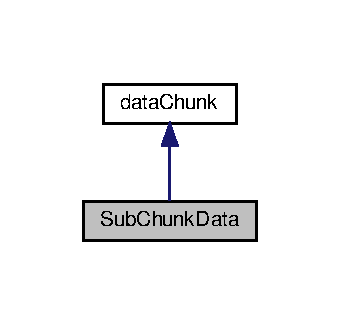
\includegraphics[width=163pt]{structSubChunkData__inherit__graph}
\end{center}
\end{figure}


Collaboration diagram for Sub\+Chunk\+Data\+:\nopagebreak
\begin{figure}[H]
\begin{center}
\leavevmode
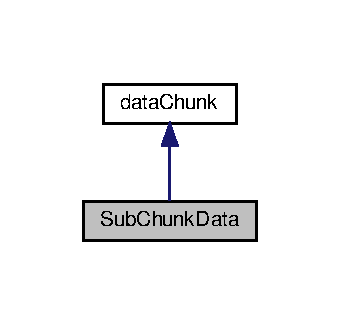
\includegraphics[width=163pt]{structSubChunkData__coll__graph}
\end{center}
\end{figure}
\subsection*{Public Attributes}
\begin{DoxyCompactItemize}
\item 
char $\ast$ \hyperlink{structSubChunkData_a8f026b9f6a0e1f74318438e61656955e}{buffer}
\end{DoxyCompactItemize}


\subsection{Detailed Description}
This is a sub chunk data to data chunk struct 

\subsection{Member Data Documentation}
\mbox{\Hypertarget{structSubChunkData_a8f026b9f6a0e1f74318438e61656955e}\label{structSubChunkData_a8f026b9f6a0e1f74318438e61656955e}} 
\index{Sub\+Chunk\+Data@{Sub\+Chunk\+Data}!buffer@{buffer}}
\index{buffer@{buffer}!Sub\+Chunk\+Data@{Sub\+Chunk\+Data}}
\subsubsection{\texorpdfstring{buffer}{buffer}}
{\footnotesize\ttfamily char$\ast$ Sub\+Chunk\+Data\+::buffer}



The documentation for this struct was generated from the following file\+:\begin{DoxyCompactItemize}
\item 
\hyperlink{wavHeader_8h}{wav\+Header.\+h}\end{DoxyCompactItemize}

\hypertarget{classWav}{}\section{Wav Class Reference}
\label{classWav}\index{Wav@{Wav}}


{\ttfamily \#include $<$wav.\+h$>$}



Collaboration diagram for Wav\+:\nopagebreak
\begin{figure}[H]
\begin{center}
\leavevmode
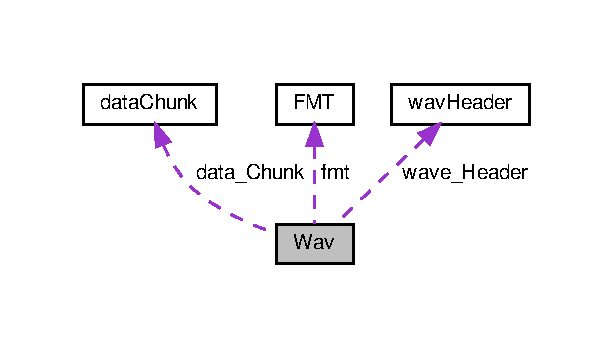
\includegraphics[width=294pt]{classWav__coll__graph}
\end{center}
\end{figure}
\subsection*{Public Member Functions}
\begin{DoxyCompactItemize}
\item 
\hyperlink{structwavHeader}{wav\+Header} \hyperlink{classWav_a5e521ff6da3e7a3ed546d948a125847f}{getwav\+Header} ()
\item 
unsigned char $\ast$ \hyperlink{classWav_a2daf07a90ed34789e3a1874973d9bd36}{get\+Buffer} ()
\item 
int \hyperlink{classWav_a11de10cb698ea0ea08f3a28580f21b39}{get\+Buffer\+Size} ()
\item 
int \hyperlink{classWav_afbd5588a3621503ee028fbec055fd075}{get\+Bit\+Depth} ()
\item 
int \hyperlink{classWav_abfc3c1b6afed8bfc43a17cbd76f8a809}{get\+Num\+Channels} ()
\item 
void \hyperlink{classWav_a8dbfa6c6dc4d8a0df92b0e4cb49d0133}{read\+File} (const std\+::string \&filename)
\item 
void \hyperlink{classWav_a3e4d48579d4c83afb0519ac8492af6d0}{write\+File} (const std\+::string \&out\+Filename)
\item 
\hyperlink{classWav_a1510b246ba121b103a60b8e7839af25f}{$\sim$\+Wav} ()
\end{DoxyCompactItemize}
\subsection*{Protected Attributes}
\begin{DoxyCompactItemize}
\item 
int \hyperlink{classWav_aaa1fc130f301f39cc74091dfb9750d13}{buffer\+Size\+\_\+data}
\item 
unsigned char $\ast$ \hyperlink{classWav_ae1ba9e10151e9d104c150f6cc5512199}{buffer} = N\+U\+LL
\item 
int \hyperlink{classWav_aaf92f0800a562d0f80783026607c8097}{bit\+Depth}
\item 
int \hyperlink{classWav_a82c5392364a4ccf8dfe725a3c7a403ec}{num\+Channels}
\item 
std\+::vector$<$ \hyperlink{structSubChunkData}{Sub\+Chunk\+Data} $>$ \hyperlink{classWav_ae6078b0bc65f5bcf4c2b7e3e7b4cf8bf}{metadata}
\item 
\hyperlink{structwavHeader}{wav\+Header} \hyperlink{classWav_a3d95345a678bba0772e48325306ecda1}{wave\+\_\+\+Header}
\item 
\hyperlink{structdataChunk}{data\+Chunk} \hyperlink{classWav_ad56011c7baf92b85b81483d7ef8b58ef}{data\+\_\+\+Chunk}
\item 
\hyperlink{structFMT}{F\+MT} \hyperlink{classWav_a2d8b662300b2821186951e428da6a6a9}{fmt}
\end{DoxyCompactItemize}


\subsection{Detailed Description}
This is a \hyperlink{classWav}{Wav} class 

\subsection{Constructor \& Destructor Documentation}
\mbox{\Hypertarget{classWav_a1510b246ba121b103a60b8e7839af25f}\label{classWav_a1510b246ba121b103a60b8e7839af25f}} 
\index{Wav@{Wav}!````~Wav@{$\sim$\+Wav}}
\index{````~Wav@{$\sim$\+Wav}!Wav@{Wav}}
\subsubsection{\texorpdfstring{$\sim$\+Wav()}{~Wav()}}
{\footnotesize\ttfamily Wav\+::$\sim$\+Wav (\begin{DoxyParamCaption}{ }\end{DoxyParamCaption})}

\hyperlink{classWav}{Wav} deconstructor 

\subsection{Member Function Documentation}
\mbox{\Hypertarget{classWav_afbd5588a3621503ee028fbec055fd075}\label{classWav_afbd5588a3621503ee028fbec055fd075}} 
\index{Wav@{Wav}!get\+Bit\+Depth@{get\+Bit\+Depth}}
\index{get\+Bit\+Depth@{get\+Bit\+Depth}!Wav@{Wav}}
\subsubsection{\texorpdfstring{get\+Bit\+Depth()}{getBitDepth()}}
{\footnotesize\ttfamily int Wav\+::get\+Bit\+Depth (\begin{DoxyParamCaption}{ }\end{DoxyParamCaption})}

Getter for bit depth \mbox{\Hypertarget{classWav_a2daf07a90ed34789e3a1874973d9bd36}\label{classWav_a2daf07a90ed34789e3a1874973d9bd36}} 
\index{Wav@{Wav}!get\+Buffer@{get\+Buffer}}
\index{get\+Buffer@{get\+Buffer}!Wav@{Wav}}
\subsubsection{\texorpdfstring{get\+Buffer()}{getBuffer()}}
{\footnotesize\ttfamily unsigned char $\ast$ Wav\+::get\+Buffer (\begin{DoxyParamCaption}{ }\end{DoxyParamCaption})}

Getter for character buffer \mbox{\Hypertarget{classWav_a11de10cb698ea0ea08f3a28580f21b39}\label{classWav_a11de10cb698ea0ea08f3a28580f21b39}} 
\index{Wav@{Wav}!get\+Buffer\+Size@{get\+Buffer\+Size}}
\index{get\+Buffer\+Size@{get\+Buffer\+Size}!Wav@{Wav}}
\subsubsection{\texorpdfstring{get\+Buffer\+Size()}{getBufferSize()}}
{\footnotesize\ttfamily int Wav\+::get\+Buffer\+Size (\begin{DoxyParamCaption}{ }\end{DoxyParamCaption})}

Getter for buffer size \mbox{\Hypertarget{classWav_abfc3c1b6afed8bfc43a17cbd76f8a809}\label{classWav_abfc3c1b6afed8bfc43a17cbd76f8a809}} 
\index{Wav@{Wav}!get\+Num\+Channels@{get\+Num\+Channels}}
\index{get\+Num\+Channels@{get\+Num\+Channels}!Wav@{Wav}}
\subsubsection{\texorpdfstring{get\+Num\+Channels()}{getNumChannels()}}
{\footnotesize\ttfamily int Wav\+::get\+Num\+Channels (\begin{DoxyParamCaption}{ }\end{DoxyParamCaption})}

Getter for number of channels \mbox{\Hypertarget{classWav_a5e521ff6da3e7a3ed546d948a125847f}\label{classWav_a5e521ff6da3e7a3ed546d948a125847f}} 
\index{Wav@{Wav}!getwav\+Header@{getwav\+Header}}
\index{getwav\+Header@{getwav\+Header}!Wav@{Wav}}
\subsubsection{\texorpdfstring{getwav\+Header()}{getwavHeader()}}
{\footnotesize\ttfamily \hyperlink{structwavHeader}{wav\+Header} Wav\+::getwav\+Header (\begin{DoxyParamCaption}{ }\end{DoxyParamCaption})}

Getter for wave\+\_\+header \mbox{\Hypertarget{classWav_a8dbfa6c6dc4d8a0df92b0e4cb49d0133}\label{classWav_a8dbfa6c6dc4d8a0df92b0e4cb49d0133}} 
\index{Wav@{Wav}!read\+File@{read\+File}}
\index{read\+File@{read\+File}!Wav@{Wav}}
\subsubsection{\texorpdfstring{read\+File()}{readFile()}}
{\footnotesize\ttfamily void Wav\+::read\+File (\begin{DoxyParamCaption}\item[{const std\+::string \&}]{filename }\end{DoxyParamCaption})}

This function reads in the file 
\begin{DoxyParams}{Parameters}
{\em filename} & -\/ string type for the file loaded \\
\hline
\end{DoxyParams}
\mbox{\Hypertarget{classWav_a3e4d48579d4c83afb0519ac8492af6d0}\label{classWav_a3e4d48579d4c83afb0519ac8492af6d0}} 
\index{Wav@{Wav}!write\+File@{write\+File}}
\index{write\+File@{write\+File}!Wav@{Wav}}
\subsubsection{\texorpdfstring{write\+File()}{writeFile()}}
{\footnotesize\ttfamily void Wav\+::write\+File (\begin{DoxyParamCaption}\item[{const std\+::string \&}]{out\+Filename }\end{DoxyParamCaption})}

This function writes in the file 
\begin{DoxyParams}{Parameters}
{\em out\+Filename} & -\/ string type for the file loaded \\
\hline
\end{DoxyParams}


\subsection{Member Data Documentation}
\mbox{\Hypertarget{classWav_aaf92f0800a562d0f80783026607c8097}\label{classWav_aaf92f0800a562d0f80783026607c8097}} 
\index{Wav@{Wav}!bit\+Depth@{bit\+Depth}}
\index{bit\+Depth@{bit\+Depth}!Wav@{Wav}}
\subsubsection{\texorpdfstring{bit\+Depth}{bitDepth}}
{\footnotesize\ttfamily int Wav\+::bit\+Depth\hspace{0.3cm}{\ttfamily [protected]}}

\mbox{\Hypertarget{classWav_ae1ba9e10151e9d104c150f6cc5512199}\label{classWav_ae1ba9e10151e9d104c150f6cc5512199}} 
\index{Wav@{Wav}!buffer@{buffer}}
\index{buffer@{buffer}!Wav@{Wav}}
\subsubsection{\texorpdfstring{buffer}{buffer}}
{\footnotesize\ttfamily unsigned char$\ast$ Wav\+::buffer = N\+U\+LL\hspace{0.3cm}{\ttfamily [protected]}}

\mbox{\Hypertarget{classWav_aaa1fc130f301f39cc74091dfb9750d13}\label{classWav_aaa1fc130f301f39cc74091dfb9750d13}} 
\index{Wav@{Wav}!buffer\+Size\+\_\+data@{buffer\+Size\+\_\+data}}
\index{buffer\+Size\+\_\+data@{buffer\+Size\+\_\+data}!Wav@{Wav}}
\subsubsection{\texorpdfstring{buffer\+Size\+\_\+data}{bufferSize\_data}}
{\footnotesize\ttfamily int Wav\+::buffer\+Size\+\_\+data\hspace{0.3cm}{\ttfamily [protected]}}

\mbox{\Hypertarget{classWav_ad56011c7baf92b85b81483d7ef8b58ef}\label{classWav_ad56011c7baf92b85b81483d7ef8b58ef}} 
\index{Wav@{Wav}!data\+\_\+\+Chunk@{data\+\_\+\+Chunk}}
\index{data\+\_\+\+Chunk@{data\+\_\+\+Chunk}!Wav@{Wav}}
\subsubsection{\texorpdfstring{data\+\_\+\+Chunk}{data\_Chunk}}
{\footnotesize\ttfamily \hyperlink{structdataChunk}{data\+Chunk} Wav\+::data\+\_\+\+Chunk\hspace{0.3cm}{\ttfamily [protected]}}

\mbox{\Hypertarget{classWav_a2d8b662300b2821186951e428da6a6a9}\label{classWav_a2d8b662300b2821186951e428da6a6a9}} 
\index{Wav@{Wav}!fmt@{fmt}}
\index{fmt@{fmt}!Wav@{Wav}}
\subsubsection{\texorpdfstring{fmt}{fmt}}
{\footnotesize\ttfamily \hyperlink{structFMT}{F\+MT} Wav\+::fmt\hspace{0.3cm}{\ttfamily [protected]}}

\mbox{\Hypertarget{classWav_ae6078b0bc65f5bcf4c2b7e3e7b4cf8bf}\label{classWav_ae6078b0bc65f5bcf4c2b7e3e7b4cf8bf}} 
\index{Wav@{Wav}!metadata@{metadata}}
\index{metadata@{metadata}!Wav@{Wav}}
\subsubsection{\texorpdfstring{metadata}{metadata}}
{\footnotesize\ttfamily std\+::vector$<$\hyperlink{structSubChunkData}{Sub\+Chunk\+Data}$>$ Wav\+::metadata\hspace{0.3cm}{\ttfamily [protected]}}

\mbox{\Hypertarget{classWav_a82c5392364a4ccf8dfe725a3c7a403ec}\label{classWav_a82c5392364a4ccf8dfe725a3c7a403ec}} 
\index{Wav@{Wav}!num\+Channels@{num\+Channels}}
\index{num\+Channels@{num\+Channels}!Wav@{Wav}}
\subsubsection{\texorpdfstring{num\+Channels}{numChannels}}
{\footnotesize\ttfamily int Wav\+::num\+Channels\hspace{0.3cm}{\ttfamily [protected]}}

\mbox{\Hypertarget{classWav_a3d95345a678bba0772e48325306ecda1}\label{classWav_a3d95345a678bba0772e48325306ecda1}} 
\index{Wav@{Wav}!wave\+\_\+\+Header@{wave\+\_\+\+Header}}
\index{wave\+\_\+\+Header@{wave\+\_\+\+Header}!Wav@{Wav}}
\subsubsection{\texorpdfstring{wave\+\_\+\+Header}{wave\_Header}}
{\footnotesize\ttfamily \hyperlink{structwavHeader}{wav\+Header} Wav\+::wave\+\_\+\+Header\hspace{0.3cm}{\ttfamily [protected]}}



The documentation for this class was generated from the following files\+:\begin{DoxyCompactItemize}
\item 
\hyperlink{wav_8h}{wav.\+h}\item 
\hyperlink{wav_8cpp}{wav.\+cpp}\end{DoxyCompactItemize}

\hypertarget{structWave__Header}{}\section{Wave\+\_\+\+Header Struct Reference}
\label{structWave__Header}\index{Wave\+\_\+\+Header@{Wave\+\_\+\+Header}}
\subsection*{Public Attributes}
\begin{DoxyCompactItemize}
\item 
\mbox{\Hypertarget{structWave__Header_ac90ed5a284cbf30b3f69ea082de3a0c6}\label{structWave__Header_ac90ed5a284cbf30b3f69ea082de3a0c6}} 
char {\bfseries riff} \mbox{[}4\mbox{]}
\item 
\mbox{\Hypertarget{structWave__Header_a6928c2d8b8904339ebb788eb8290f142}\label{structWave__Header_a6928c2d8b8904339ebb788eb8290f142}} 
int {\bfseries wav\+Size}
\item 
\mbox{\Hypertarget{structWave__Header_a0619c4f802e42c1f0df93f77eab026b3}\label{structWave__Header_a0619c4f802e42c1f0df93f77eab026b3}} 
char {\bfseries wave} \mbox{[}4\mbox{]}
\item 
\mbox{\Hypertarget{structWave__Header_a14d810235149a0b8bfab223852e1d414}\label{structWave__Header_a14d810235149a0b8bfab223852e1d414}} 
char {\bfseries fmt} \mbox{[}4\mbox{]}
\item 
\mbox{\Hypertarget{structWave__Header_a6b4c3112066ec18881997ca2f42b9c53}\label{structWave__Header_a6b4c3112066ec18881997ca2f42b9c53}} 
int {\bfseries fmt\+Chunk\+Size}
\item 
\mbox{\Hypertarget{structWave__Header_a78581f9b4fa8ccd937260f6acd1805e4}\label{structWave__Header_a78581f9b4fa8ccd937260f6acd1805e4}} 
short {\bfseries audio\+Format}
\item 
\mbox{\Hypertarget{structWave__Header_a06db23d3c3ae3e20dca44ec8e1b62210}\label{structWave__Header_a06db23d3c3ae3e20dca44ec8e1b62210}} 
short {\bfseries num\+Channels}
\item 
\mbox{\Hypertarget{structWave__Header_ab5fb0a7055f8ea82df946d215bc803ee}\label{structWave__Header_ab5fb0a7055f8ea82df946d215bc803ee}} 
int {\bfseries sample\+Rate}
\item 
\mbox{\Hypertarget{structWave__Header_ad060843c06006ec4158afc8dccea9fc3}\label{structWave__Header_ad060843c06006ec4158afc8dccea9fc3}} 
int {\bfseries byte\+Rate}
\item 
\mbox{\Hypertarget{structWave__Header_aa9440351df7a8f57a5536fea94958c56}\label{structWave__Header_aa9440351df7a8f57a5536fea94958c56}} 
short {\bfseries sample\+Alignment}
\item 
\mbox{\Hypertarget{structWave__Header_a84a83027dfbce3d40ef313e2e51fb14c}\label{structWave__Header_a84a83027dfbce3d40ef313e2e51fb14c}} 
short {\bfseries bit\+Depth}
\item 
\mbox{\Hypertarget{structWave__Header_a4e2bc40c58a9da8bbe53b14e9f822153}\label{structWave__Header_a4e2bc40c58a9da8bbe53b14e9f822153}} 
char {\bfseries data\+\_\+header} \mbox{[}4\mbox{]}
\item 
\mbox{\Hypertarget{structWave__Header_a30a52cd01475ca214d183dfb1d6c4230}\label{structWave__Header_a30a52cd01475ca214d183dfb1d6c4230}} 
int {\bfseries data\+\_\+bytes}
\end{DoxyCompactItemize}


The documentation for this struct was generated from the following file\+:\begin{DoxyCompactItemize}
\item 
Wave\+\_\+\+Header.\+h\end{DoxyCompactItemize}

\hypertarget{structwavHeader}{}\section{wav\+Header Struct Reference}
\label{structwavHeader}\index{wav\+Header@{wav\+Header}}


{\ttfamily \#include $<$wav\+Header.\+h$>$}

\subsection*{Public Attributes}
\begin{DoxyCompactItemize}
\item 
char \hyperlink{structwavHeader_aa001e48dfa6193b32562533ad119c60d}{riff\+\_\+header} \mbox{[}4\mbox{]}
\item 
char \hyperlink{structwavHeader_ae9a0bfdec6e8b7ba48dd27d7ac587f62}{wave\+\_\+header} \mbox{[}4\mbox{]}
\item 
int \hyperlink{structwavHeader_adf513d299b6989b3046347077e077c82}{wav\+\_\+size}
\end{DoxyCompactItemize}


\subsection{Detailed Description}
This is a Wave Header struct 

\subsection{Member Data Documentation}
\mbox{\Hypertarget{structwavHeader_aa001e48dfa6193b32562533ad119c60d}\label{structwavHeader_aa001e48dfa6193b32562533ad119c60d}} 
\index{wav\+Header@{wav\+Header}!riff\+\_\+header@{riff\+\_\+header}}
\index{riff\+\_\+header@{riff\+\_\+header}!wav\+Header@{wav\+Header}}
\subsubsection{\texorpdfstring{riff\+\_\+header}{riff\_header}}
{\footnotesize\ttfamily char wav\+Header\+::riff\+\_\+header\mbox{[}4\mbox{]}}

\mbox{\Hypertarget{structwavHeader_adf513d299b6989b3046347077e077c82}\label{structwavHeader_adf513d299b6989b3046347077e077c82}} 
\index{wav\+Header@{wav\+Header}!wav\+\_\+size@{wav\+\_\+size}}
\index{wav\+\_\+size@{wav\+\_\+size}!wav\+Header@{wav\+Header}}
\subsubsection{\texorpdfstring{wav\+\_\+size}{wav\_size}}
{\footnotesize\ttfamily int wav\+Header\+::wav\+\_\+size}

\mbox{\Hypertarget{structwavHeader_ae9a0bfdec6e8b7ba48dd27d7ac587f62}\label{structwavHeader_ae9a0bfdec6e8b7ba48dd27d7ac587f62}} 
\index{wav\+Header@{wav\+Header}!wave\+\_\+header@{wave\+\_\+header}}
\index{wave\+\_\+header@{wave\+\_\+header}!wav\+Header@{wav\+Header}}
\subsubsection{\texorpdfstring{wave\+\_\+header}{wave\_header}}
{\footnotesize\ttfamily char wav\+Header\+::wave\+\_\+header\mbox{[}4\mbox{]}}



The documentation for this struct was generated from the following file\+:\begin{DoxyCompactItemize}
\item 
\hyperlink{wavHeader_8h}{wav\+Header.\+h}\end{DoxyCompactItemize}

\chapter{File Documentation}
\hypertarget{echo_8cpp}{}\section{echo.\+cpp File Reference}
\label{echo_8cpp}\index{echo.\+cpp@{echo.\+cpp}}
{\ttfamily \#include \char`\"{}echo.\+h\char`\"{}}\newline
{\ttfamily \#include $<$cmath$>$}\newline
Include dependency graph for echo.\+cpp\+:\nopagebreak
\begin{figure}[H]
\begin{center}
\leavevmode
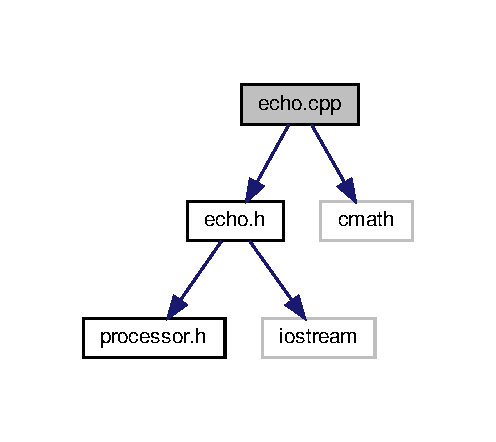
\includegraphics[width=238pt]{echo_8cpp__incl}
\end{center}
\end{figure}

\hypertarget{echo_8h}{}\section{echo.\+h File Reference}
\label{echo_8h}\index{echo.\+h@{echo.\+h}}
{\ttfamily \#include \char`\"{}processor.\+h\char`\"{}}\newline
{\ttfamily \#include $<$iostream$>$}\newline
Include dependency graph for echo.\+h\+:\nopagebreak
\begin{figure}[H]
\begin{center}
\leavevmode
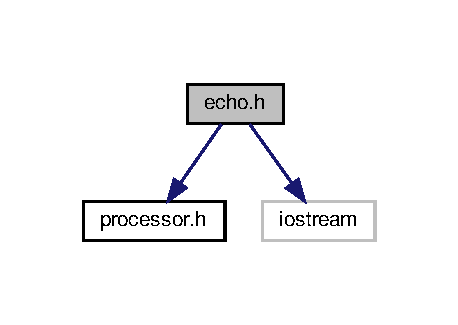
\includegraphics[width=220pt]{echo_8h__incl}
\end{center}
\end{figure}
This graph shows which files directly or indirectly include this file\+:\nopagebreak
\begin{figure}[H]
\begin{center}
\leavevmode
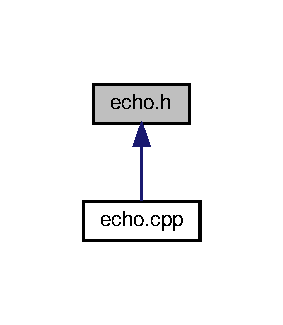
\includegraphics[width=136pt]{echo_8h__dep__incl}
\end{center}
\end{figure}
\subsection*{Classes}
\begin{DoxyCompactItemize}
\item 
class \hyperlink{classEcho}{Echo}
\end{DoxyCompactItemize}

\hypertarget{echo__diag_8h}{}\section{echo\+\_\+diag.\+h File Reference}
\label{echo__diag_8h}\index{echo\+\_\+diag.\+h@{echo\+\_\+diag.\+h}}
{\ttfamily \#include \char`\"{}processor.\+h\char`\"{}}\newline
Include dependency graph for echo\+\_\+diag.\+h\+:\nopagebreak
\begin{figure}[H]
\begin{center}
\leavevmode
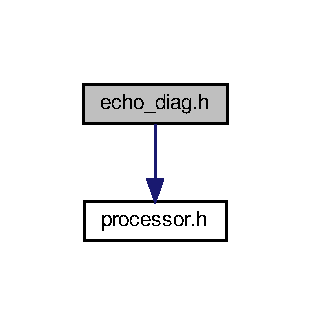
\includegraphics[width=149pt]{echo__diag_8h__incl}
\end{center}
\end{figure}
\subsection*{Classes}
\begin{DoxyCompactItemize}
\item 
class \hyperlink{classEcho}{Echo}
\end{DoxyCompactItemize}

\hypertarget{main_8cpp}{}\section{main.\+cpp File Reference}
\label{main_8cpp}\index{main.\+cpp@{main.\+cpp}}
{\ttfamily \#include $<$iostream$>$}\newline
{\ttfamily \#include $<$fstream$>$}\newline
{\ttfamily \#include $<$string$>$}\newline
{\ttfamily \#include $<$vector$>$}\newline
{\ttfamily \#include \char`\"{}Wave\+\_\+\+Header.\+h\char`\"{}}\newline
Include dependency graph for main.\+cpp\+:

\hypertarget{maincopy_8cpp}{}\section{maincopy.\+cpp File Reference}
\label{maincopy_8cpp}\index{maincopy.\+cpp@{maincopy.\+cpp}}
{\ttfamily \#include $<$iostream$>$}\newline
{\ttfamily \#include $<$fstream$>$}\newline
{\ttfamily \#include $<$string$>$}\newline
{\ttfamily \#include $<$vector$>$}\newline
{\ttfamily \#include \char`\"{}Wave\+\_\+\+Header.\+h\char`\"{}}\newline
Include dependency graph for maincopy.\+cpp\+:\nopagebreak
\begin{figure}[H]
\begin{center}
\leavevmode
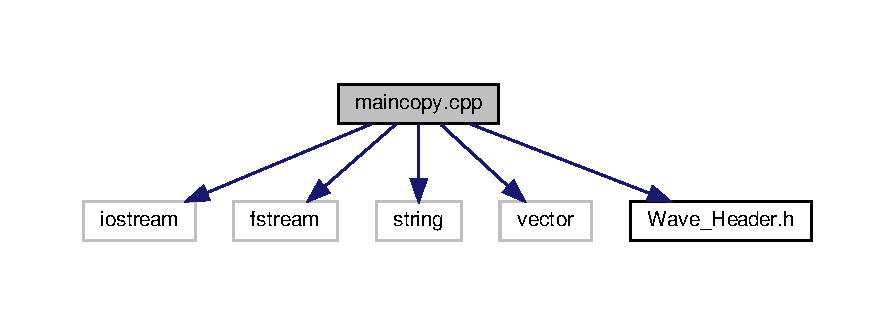
\includegraphics[width=350pt]{maincopy_8cpp__incl}
\end{center}
\end{figure}
\subsection*{Functions}
\begin{DoxyCompactItemize}
\item 
Draft of C\+SV writing file name and data columns bool \hyperlink{maincopy_8cpp_ab788ef71dec44feec2734b4f074e0c00}{write\+Datato\+File} (string file\+\_\+name, string data\+\_\+one, string data\+\_\+two)
\item 
to sta int \hyperlink{maincopy_8cpp_af0aa598edfa8d4f944abef9fc6144248}{main} (int argc, char $\ast$argv\mbox{[}$\,$\mbox{]})
\item 
\hyperlink{maincopy_8cpp_af9dc4627bb719323ede8dc29ef10c6cf}{for} (int i=0;i$<$=\hyperlink{maincopy_8cpp_a96698bc868ee1ce110d30d95ea607633}{number\+Of\+Files};i++)
\end{DoxyCompactItemize}
\subsection*{Variables}
\begin{DoxyCompactItemize}
\item 
to \hyperlink{maincopy_8cpp_ac3dae6f73da5fd8952a735f56fc6660d}{input}
\item 
out Data cout$<$$<$ \char`\"{}File is \+:\char`\"{}$<$$<$ filelength$<$$<$ \char`\"{} bytes.\char`\"{}$<$$<$ endl;cout$<$$<$ \char`\"{}R\+I\+FF header \+:\char`\"{}$<$$<$ wav\+Header.\+R\+I\+FF\mbox{[}0\mbox{]}$<$$<$ wav\+Header.\+R\+I\+FF\mbox{[}1\mbox{]}$<$$<$ wav\+Header.\+R\+I\+FF\mbox{[}2\mbox{]}$<$$<$ wav\+Header.\+R\+I\+FF\mbox{[}3\mbox{]}$<$$<$ endl;cout$<$$<$ \char`\"{}W\+A\+VE header \+:\char`\"{}$<$$<$ wav\+Header.\+W\+A\+VE\mbox{[}0\mbox{]}$<$$<$ wav\+Header.\+W\+A\+VE\mbox{[}1\mbox{]}$<$$<$ wav\+Header.\+W\+A\+VE\mbox{[}2\mbox{]}$<$$<$ wav\+Header.\+W\+A\+VE\mbox{[}3\mbox{]}$<$$<$ endl;cout$<$$<$ \char`\"{}F\+MT \+:\char`\"{}$<$$<$ wav\+Header.\+fmt\mbox{[}0\mbox{]}$<$$<$ wav\+Header.\+fmt\mbox{[}1\mbox{]}$<$$<$ wav\+Header.\+fmt\mbox{[}2\mbox{]}$<$$<$ wav\+Header.\+fmt\mbox{[}3\mbox{]}$<$$<$ endl;cout$<$$<$ \char`\"{}Data size \+:\char`\"{}$<$$<$ wav\+Header.\+Chunk\+Size$<$$<$ endl;int user\+InputC;cout$<$$<$ \char`\"{}How many processors would you like to use?\char`\"{}$<$$<$ endl;cin $>$ \hyperlink{maincopy_8cpp_a05aa176620acf40683fe4d9bbad98172}{user\+InputC}
\item 
int \hyperlink{maincopy_8cpp_a96698bc868ee1ce110d30d95ea607633}{number\+Of\+Files}
\end{DoxyCompactItemize}


\subsection{Function Documentation}
\mbox{\Hypertarget{maincopy_8cpp_af9dc4627bb719323ede8dc29ef10c6cf}\label{maincopy_8cpp_af9dc4627bb719323ede8dc29ef10c6cf}} 
\index{maincopy.\+cpp@{maincopy.\+cpp}!for@{for}}
\index{for@{for}!maincopy.\+cpp@{maincopy.\+cpp}}
\subsubsection{\texorpdfstring{for()}{for()}}
{\footnotesize\ttfamily for (\begin{DoxyParamCaption}\item[{int}]{i = {\ttfamily 0;~i~$<$=~\hyperlink{maincopy_8cpp_a96698bc868ee1ce110d30d95ea607633}{number\+Of\+Files};~i++} }\end{DoxyParamCaption})}

\mbox{\Hypertarget{maincopy_8cpp_af0aa598edfa8d4f944abef9fc6144248}\label{maincopy_8cpp_af0aa598edfa8d4f944abef9fc6144248}} 
\index{maincopy.\+cpp@{maincopy.\+cpp}!main@{main}}
\index{main@{main}!maincopy.\+cpp@{maincopy.\+cpp}}
\subsubsection{\texorpdfstring{main()}{main()}}
{\footnotesize\ttfamily to sta int main (\begin{DoxyParamCaption}\item[{int}]{argc,  }\item[{char $\ast$}]{argv\mbox{[}$\,$\mbox{]} }\end{DoxyParamCaption})}

Here is the call graph for this function\+:\nopagebreak
\begin{figure}[H]
\begin{center}
\leavevmode
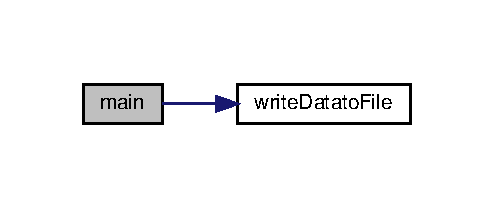
\includegraphics[width=237pt]{maincopy_8cpp_af0aa598edfa8d4f944abef9fc6144248_cgraph}
\end{center}
\end{figure}
\mbox{\Hypertarget{maincopy_8cpp_ab788ef71dec44feec2734b4f074e0c00}\label{maincopy_8cpp_ab788ef71dec44feec2734b4f074e0c00}} 
\index{maincopy.\+cpp@{maincopy.\+cpp}!write\+Datato\+File@{write\+Datato\+File}}
\index{write\+Datato\+File@{write\+Datato\+File}!maincopy.\+cpp@{maincopy.\+cpp}}
\subsubsection{\texorpdfstring{write\+Datato\+File()}{writeDatatoFile()}}
{\footnotesize\ttfamily Draft of C\+SV writing file name and data columns bool write\+Datato\+File (\begin{DoxyParamCaption}\item[{string}]{file\+\_\+name,  }\item[{string}]{data\+\_\+one,  }\item[{string}]{data\+\_\+two }\end{DoxyParamCaption})}

Here is the caller graph for this function\+:\nopagebreak
\begin{figure}[H]
\begin{center}
\leavevmode
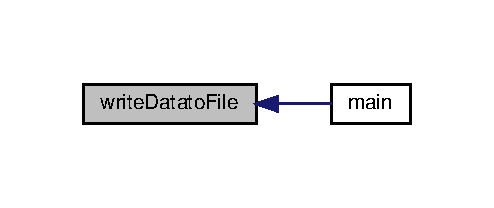
\includegraphics[width=237pt]{maincopy_8cpp_ab788ef71dec44feec2734b4f074e0c00_icgraph}
\end{center}
\end{figure}


\subsection{Variable Documentation}
\mbox{\Hypertarget{maincopy_8cpp_ac3dae6f73da5fd8952a735f56fc6660d}\label{maincopy_8cpp_ac3dae6f73da5fd8952a735f56fc6660d}} 
\index{maincopy.\+cpp@{maincopy.\+cpp}!input@{input}}
\index{input@{input}!maincopy.\+cpp@{maincopy.\+cpp}}
\subsubsection{\texorpdfstring{input}{input}}
{\footnotesize\ttfamily to input}

\mbox{\Hypertarget{maincopy_8cpp_a96698bc868ee1ce110d30d95ea607633}\label{maincopy_8cpp_a96698bc868ee1ce110d30d95ea607633}} 
\index{maincopy.\+cpp@{maincopy.\+cpp}!number\+Of\+Files@{number\+Of\+Files}}
\index{number\+Of\+Files@{number\+Of\+Files}!maincopy.\+cpp@{maincopy.\+cpp}}
\subsubsection{\texorpdfstring{number\+Of\+Files}{numberOfFiles}}
{\footnotesize\ttfamily cout$<$$<$ \char`\"{}How many files would you like to process?\char`\"{} $<$$<$ endl;cin $>$ number\+Of\+Files}

\mbox{\Hypertarget{maincopy_8cpp_a05aa176620acf40683fe4d9bbad98172}\label{maincopy_8cpp_a05aa176620acf40683fe4d9bbad98172}} 
\index{maincopy.\+cpp@{maincopy.\+cpp}!user\+InputC@{user\+InputC}}
\index{user\+InputC@{user\+InputC}!maincopy.\+cpp@{maincopy.\+cpp}}
\subsubsection{\texorpdfstring{user\+InputC}{userInputC}}
{\footnotesize\ttfamily out Data cout$<$$<$ \char`\"{}File is \+:\char`\"{} $<$$<$ filelength $<$$<$ \char`\"{} bytes.\char`\"{} $<$$<$ endl; cout $<$$<$ \char`\"{}R\+I\+FF header \+:\char`\"{} $<$$<$ wav\+Header.\+R\+I\+FF\mbox{[}0\mbox{]} $<$$<$ wav\+Header.\+R\+I\+FF\mbox{[}1\mbox{]} $<$$<$ wav\+Header.\+R\+I\+FF\mbox{[}2\mbox{]} $<$$<$ wav\+Header.\+R\+I\+FF\mbox{[}3\mbox{]} $<$$<$ endl; cout $<$$<$ \char`\"{}W\+A\+VE header \+:\char`\"{} $<$$<$ wav\+Header.\+W\+A\+VE\mbox{[}0\mbox{]} $<$$<$ wav\+Header.\+W\+A\+VE\mbox{[}1\mbox{]} $<$$<$ wav\+Header.\+W\+A\+VE\mbox{[}2\mbox{]} $<$$<$ wav\+Header.\+W\+A\+VE\mbox{[}3\mbox{]} $<$$<$ endl; cout $<$$<$ \char`\"{}F\+MT \+:\char`\"{} $<$$<$ wav\+Header.\+fmt\mbox{[}0\mbox{]} $<$$<$ wav\+Header.\+fmt\mbox{[}1\mbox{]} $<$$<$ wav\+Header.\+fmt\mbox{[}2\mbox{]} $<$$<$ wav\+Header.\+fmt\mbox{[}3\mbox{]} $<$$<$ endl; cout $<$$<$ \char`\"{}Data size \+:\char`\"{} $<$$<$ wav\+Header.\+Chunk\+Size $<$$<$ endl;int user\+InputC;cout $<$$<$ \char`\"{}How many processors would you like to use?\char`\"{} $<$$<$ endl;cin $>$ user\+InputC}


\hypertarget{menu_8cpp}{}\section{menu.\+cpp File Reference}
\label{menu_8cpp}\index{menu.\+cpp@{menu.\+cpp}}
{\ttfamily \#include \char`\"{}menu.\+h\char`\"{}}\newline
Include dependency graph for menu.\+cpp\+:\nopagebreak
\begin{figure}[H]
\begin{center}
\leavevmode
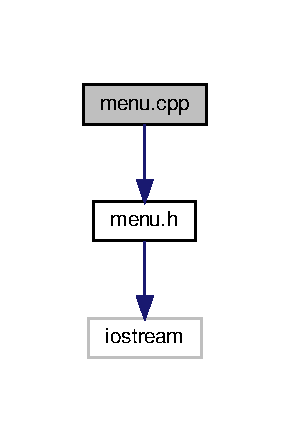
\includegraphics[width=139pt]{menu_8cpp__incl}
\end{center}
\end{figure}

\hypertarget{menu_8h}{}\section{menu.\+h File Reference}
\label{menu_8h}\index{menu.\+h@{menu.\+h}}
{\ttfamily \#include $<$iostream$>$}\newline
Include dependency graph for menu.\+h\+:\nopagebreak
\begin{figure}[H]
\begin{center}
\leavevmode
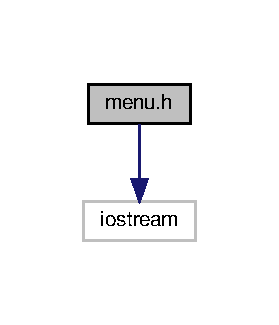
\includegraphics[width=134pt]{menu_8h__incl}
\end{center}
\end{figure}
This graph shows which files directly or indirectly include this file\+:\nopagebreak
\begin{figure}[H]
\begin{center}
\leavevmode
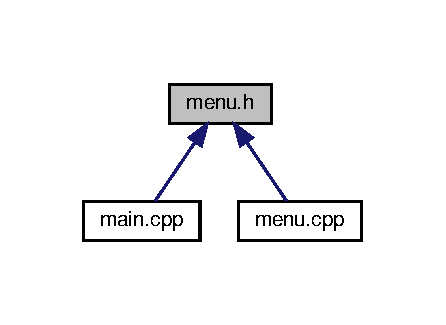
\includegraphics[width=214pt]{menu_8h__dep__incl}
\end{center}
\end{figure}
\subsection*{Classes}
\begin{DoxyCompactItemize}
\item 
class \hyperlink{classmenu}{menu$<$ T $>$}
\end{DoxyCompactItemize}

\hypertarget{metaData_8cpp}{}\section{meta\+Data.\+cpp File Reference}
\label{metaData_8cpp}\index{meta\+Data.\+cpp@{meta\+Data.\+cpp}}
{\ttfamily \#include \char`\"{}meta\+Data.\+h\char`\"{}}\newline
Include dependency graph for meta\+Data.\+cpp\+:\nopagebreak
\begin{figure}[H]
\begin{center}
\leavevmode
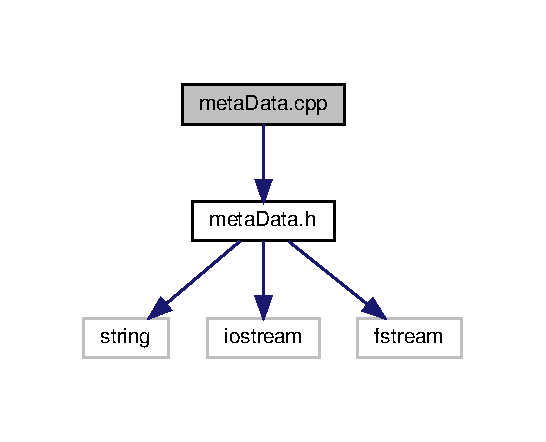
\includegraphics[width=262pt]{metaData_8cpp__incl}
\end{center}
\end{figure}
\subsection*{Functions}
\begin{DoxyCompactItemize}
\item 
\hyperlink{metaData_8cpp_a057bfd5981c207f770fa429635909a84}{for} (char chunk\+:md\+ID)
\item 
str \hyperlink{metaData_8cpp_a1f31e462e2421b2f83883e512dc768d6}{push\+\_\+back} (\textquotesingle{}\textbackslash{}0\textquotesingle{})
\end{DoxyCompactItemize}
\subsection*{Variables}
\begin{DoxyCompactItemize}
\item 
return \hyperlink{metaData_8cpp_a3e331b7cf11229d187b33cf3037e4615}{dstring}
\end{DoxyCompactItemize}


\subsection{Function Documentation}
\mbox{\Hypertarget{metaData_8cpp_a057bfd5981c207f770fa429635909a84}\label{metaData_8cpp_a057bfd5981c207f770fa429635909a84}} 
\index{meta\+Data.\+cpp@{meta\+Data.\+cpp}!for@{for}}
\index{for@{for}!meta\+Data.\+cpp@{meta\+Data.\+cpp}}
\subsubsection{\texorpdfstring{for()}{for()}}
{\footnotesize\ttfamily for (\begin{DoxyParamCaption}\item[{char chunk\+:md\+ID}]{ }\end{DoxyParamCaption})}

\mbox{\Hypertarget{metaData_8cpp_a1f31e462e2421b2f83883e512dc768d6}\label{metaData_8cpp_a1f31e462e2421b2f83883e512dc768d6}} 
\index{meta\+Data.\+cpp@{meta\+Data.\+cpp}!push\+\_\+back@{push\+\_\+back}}
\index{push\+\_\+back@{push\+\_\+back}!meta\+Data.\+cpp@{meta\+Data.\+cpp}}
\subsubsection{\texorpdfstring{push\+\_\+back()}{push\_back()}}
{\footnotesize\ttfamily str push\+\_\+back (\begin{DoxyParamCaption}\item[{\textquotesingle{}\textbackslash{}0\textquotesingle{}}]{ }\end{DoxyParamCaption})}



\subsection{Variable Documentation}
\mbox{\Hypertarget{metaData_8cpp_a3e331b7cf11229d187b33cf3037e4615}\label{metaData_8cpp_a3e331b7cf11229d187b33cf3037e4615}} 
\index{meta\+Data.\+cpp@{meta\+Data.\+cpp}!dstring@{dstring}}
\index{dstring@{dstring}!meta\+Data.\+cpp@{meta\+Data.\+cpp}}
\subsubsection{\texorpdfstring{dstring}{dstring}}
{\footnotesize\ttfamily return dstring}


\hypertarget{metaData_8h}{}\section{meta\+Data.\+h File Reference}
\label{metaData_8h}\index{meta\+Data.\+h@{meta\+Data.\+h}}
{\ttfamily \#include $<$string$>$}\newline
{\ttfamily \#include $<$iostream$>$}\newline
{\ttfamily \#include $<$fstream$>$}\newline
Include dependency graph for meta\+Data.\+h\+:\nopagebreak
\begin{figure}[H]
\begin{center}
\leavevmode
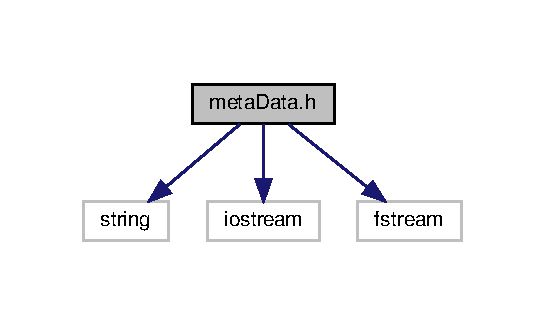
\includegraphics[width=262pt]{metaData_8h__incl}
\end{center}
\end{figure}
This graph shows which files directly or indirectly include this file\+:\nopagebreak
\begin{figure}[H]
\begin{center}
\leavevmode
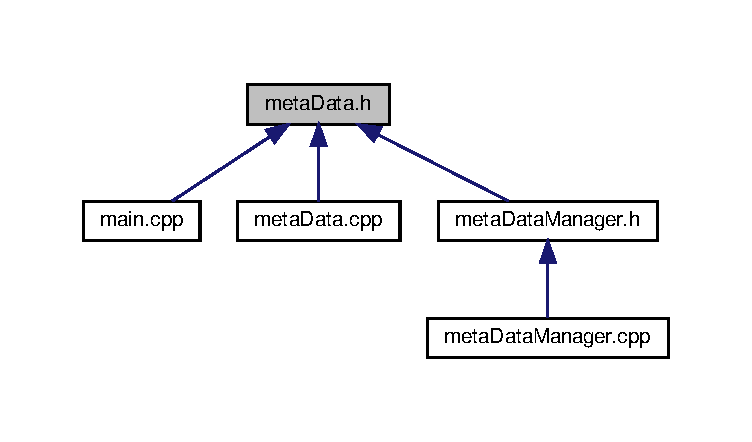
\includegraphics[width=350pt]{metaData_8h__dep__incl}
\end{center}
\end{figure}
\subsection*{Classes}
\begin{DoxyCompactItemize}
\item 
class \hyperlink{classMetaData}{Meta\+Data}
\end{DoxyCompactItemize}

\hypertarget{metaDataHeader_8h}{}\section{meta\+Data\+Header.\+h File Reference}
\label{metaDataHeader_8h}\index{meta\+Data\+Header.\+h@{meta\+Data\+Header.\+h}}
This graph shows which files directly or indirectly include this file\+:\nopagebreak
\begin{figure}[H]
\begin{center}
\leavevmode
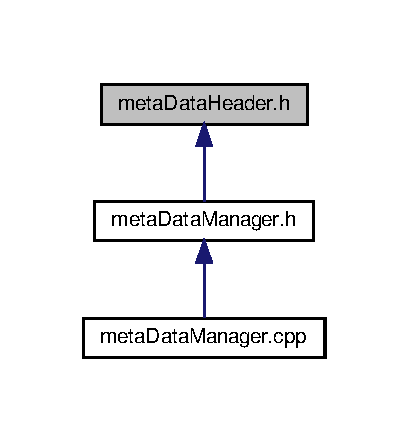
\includegraphics[width=196pt]{metaDataHeader_8h__dep__incl}
\end{center}
\end{figure}
\subsection*{Classes}
\begin{DoxyCompactItemize}
\item 
struct \hyperlink{structMetaDataHeader}{Meta\+Data\+Header}
\end{DoxyCompactItemize}

\hypertarget{metaDataManager_8cpp}{}\section{meta\+Data\+Manager.\+cpp File Reference}
\label{metaDataManager_8cpp}\index{meta\+Data\+Manager.\+cpp@{meta\+Data\+Manager.\+cpp}}
{\ttfamily \#include \char`\"{}meta\+Data\+Manager.\+h\char`\"{}}\newline
Include dependency graph for meta\+Data\+Manager.\+cpp\+:\nopagebreak
\begin{figure}[H]
\begin{center}
\leavevmode
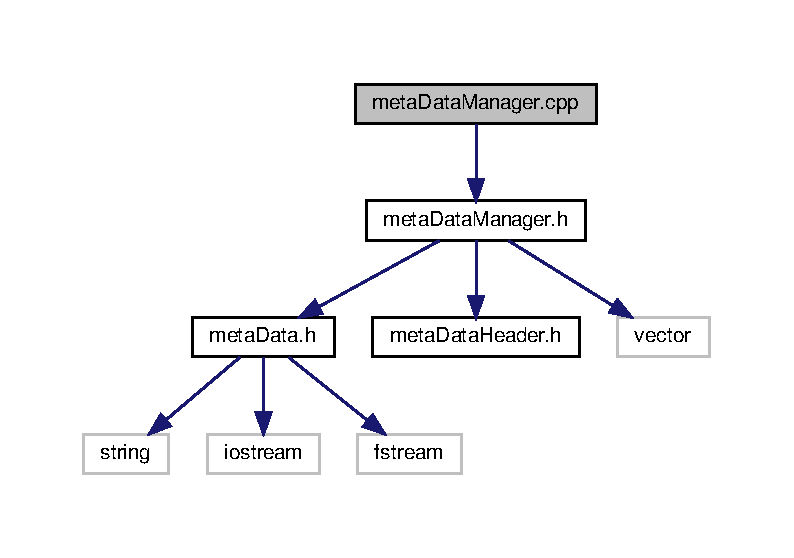
\includegraphics[width=350pt]{metaDataManager_8cpp__incl}
\end{center}
\end{figure}

\hypertarget{metaDataManager_8h}{}\section{meta\+Data\+Manager.\+h File Reference}
\label{metaDataManager_8h}\index{meta\+Data\+Manager.\+h@{meta\+Data\+Manager.\+h}}
{\ttfamily \#include \char`\"{}meta\+Data.\+h\char`\"{}}\newline
{\ttfamily \#include \char`\"{}meta\+Data\+Header.\+h\char`\"{}}\newline
{\ttfamily \#include $<$vector$>$}\newline
Include dependency graph for meta\+Data\+Manager.\+h\+:\nopagebreak
\begin{figure}[H]
\begin{center}
\leavevmode
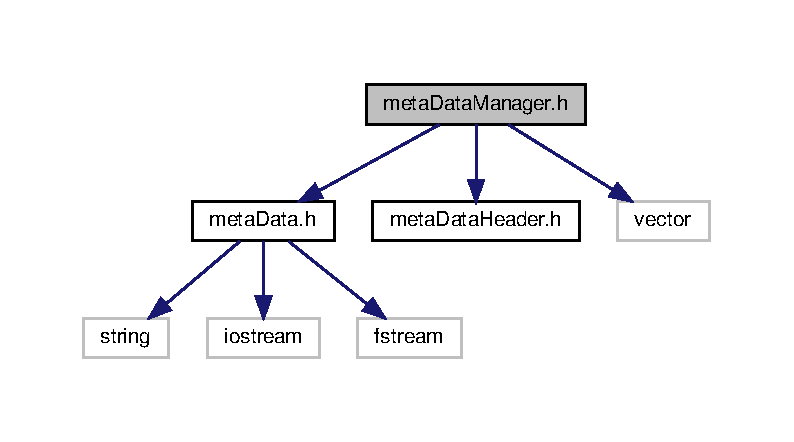
\includegraphics[width=350pt]{metaDataManager_8h__incl}
\end{center}
\end{figure}
This graph shows which files directly or indirectly include this file\+:\nopagebreak
\begin{figure}[H]
\begin{center}
\leavevmode
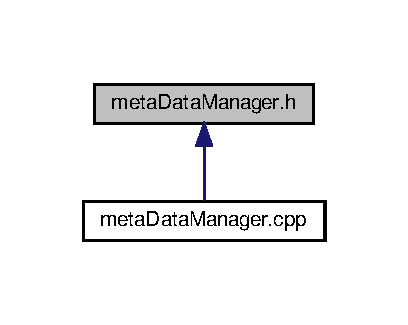
\includegraphics[width=196pt]{metaDataManager_8h__dep__incl}
\end{center}
\end{figure}
\subsection*{Classes}
\begin{DoxyCompactItemize}
\item 
class \hyperlink{classMdManager}{Md\+Manager}
\end{DoxyCompactItemize}

\hypertarget{noiseg__diag_8h}{}\section{noiseg\+\_\+diag.\+h File Reference}
\label{noiseg__diag_8h}\index{noiseg\+\_\+diag.\+h@{noiseg\+\_\+diag.\+h}}
{\ttfamily \#include \char`\"{}processor.\+h\char`\"{}}\newline
Include dependency graph for noiseg\+\_\+diag.\+h\+:\nopagebreak
\begin{figure}[H]
\begin{center}
\leavevmode
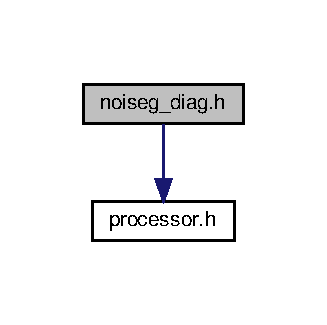
\includegraphics[width=157pt]{noiseg__diag_8h__incl}
\end{center}
\end{figure}
\subsection*{Classes}
\begin{DoxyCompactItemize}
\item 
class \hyperlink{classNoiseGate}{Noise\+Gate}
\end{DoxyCompactItemize}

\hypertarget{noiseGate_8cpp}{}\section{noise\+Gate.\+cpp File Reference}
\label{noiseGate_8cpp}\index{noise\+Gate.\+cpp@{noise\+Gate.\+cpp}}
{\ttfamily \#include \char`\"{}noise\+Gate.\+h\char`\"{}}\newline
Include dependency graph for noise\+Gate.\+cpp\+:\nopagebreak
\begin{figure}[H]
\begin{center}
\leavevmode
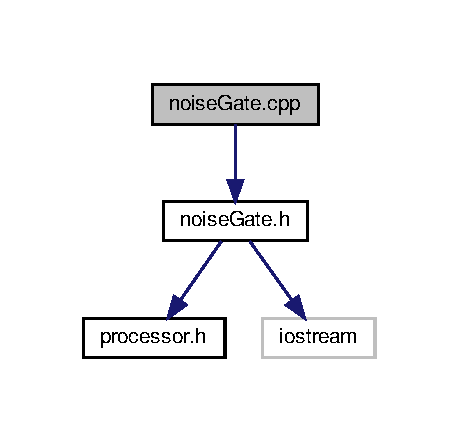
\includegraphics[width=220pt]{noiseGate_8cpp__incl}
\end{center}
\end{figure}

\hypertarget{noiseGate_8h}{}\section{noise\+Gate.\+h File Reference}
\label{noiseGate_8h}\index{noise\+Gate.\+h@{noise\+Gate.\+h}}
{\ttfamily \#include \char`\"{}processor.\+h\char`\"{}}\newline
{\ttfamily \#include $<$iostream$>$}\newline
Include dependency graph for noise\+Gate.\+h\+:\nopagebreak
\begin{figure}[H]
\begin{center}
\leavevmode
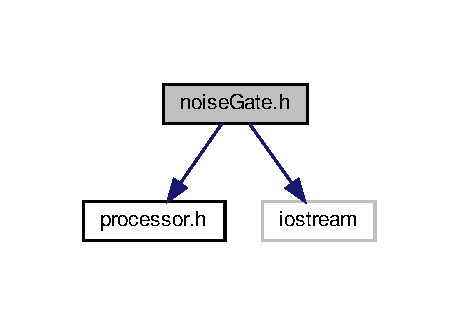
\includegraphics[width=220pt]{noiseGate_8h__incl}
\end{center}
\end{figure}
This graph shows which files directly or indirectly include this file\+:\nopagebreak
\begin{figure}[H]
\begin{center}
\leavevmode
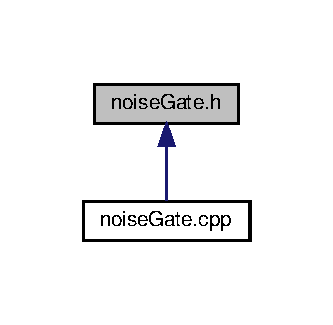
\includegraphics[width=160pt]{noiseGate_8h__dep__incl}
\end{center}
\end{figure}
\subsection*{Classes}
\begin{DoxyCompactItemize}
\item 
class \hyperlink{classNoiseGate}{Noise\+Gate}
\end{DoxyCompactItemize}

\hypertarget{norm__diag_8h}{}\section{norm\+\_\+diag.\+h File Reference}
\label{norm__diag_8h}\index{norm\+\_\+diag.\+h@{norm\+\_\+diag.\+h}}
{\ttfamily \#include \char`\"{}processor.\+h\char`\"{}}\newline
Include dependency graph for norm\+\_\+diag.\+h\+:\nopagebreak
\begin{figure}[H]
\begin{center}
\leavevmode
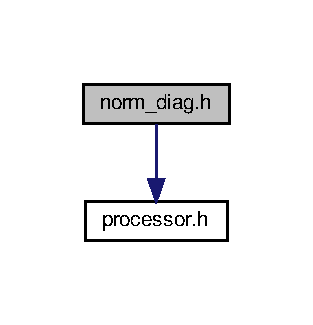
\includegraphics[width=150pt]{norm__diag_8h__incl}
\end{center}
\end{figure}
\subsection*{Classes}
\begin{DoxyCompactItemize}
\item 
class \hyperlink{classNormalization}{Normalization}
\end{DoxyCompactItemize}

\hypertarget{normalization_8cpp}{}\section{normalization.\+cpp File Reference}
\label{normalization_8cpp}\index{normalization.\+cpp@{normalization.\+cpp}}
{\ttfamily \#include \char`\"{}normalization.\+h\char`\"{}}\newline
Include dependency graph for normalization.\+cpp\+:\nopagebreak
\begin{figure}[H]
\begin{center}
\leavevmode
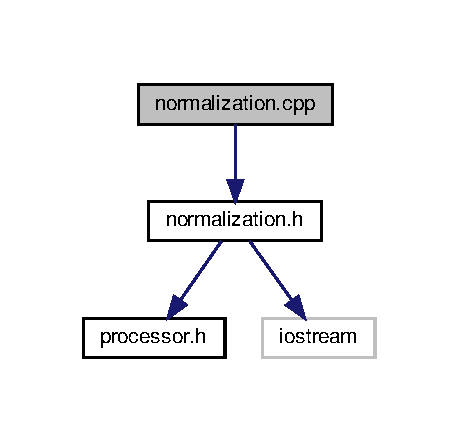
\includegraphics[width=220pt]{normalization_8cpp__incl}
\end{center}
\end{figure}

\hypertarget{normalization_8h}{}\section{normalization.\+h File Reference}
\label{normalization_8h}\index{normalization.\+h@{normalization.\+h}}
{\ttfamily \#include \char`\"{}processor.\+h\char`\"{}}\newline
{\ttfamily \#include $<$iostream$>$}\newline
Include dependency graph for normalization.\+h\+:\nopagebreak
\begin{figure}[H]
\begin{center}
\leavevmode
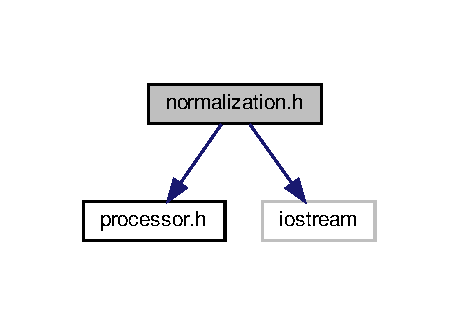
\includegraphics[width=220pt]{normalization_8h__incl}
\end{center}
\end{figure}
This graph shows which files directly or indirectly include this file\+:\nopagebreak
\begin{figure}[H]
\begin{center}
\leavevmode
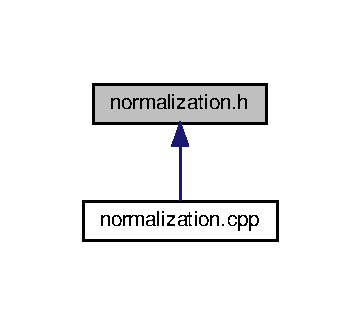
\includegraphics[width=173pt]{normalization_8h__dep__incl}
\end{center}
\end{figure}
\subsection*{Classes}
\begin{DoxyCompactItemize}
\item 
class \hyperlink{classNormalization}{Normalization}
\end{DoxyCompactItemize}

\hypertarget{Processor_8cpp}{}\section{Processor.\+cpp File Reference}
\label{Processor_8cpp}\index{Processor.\+cpp@{Processor.\+cpp}}
{\ttfamily \#include \char`\"{}Processor.\+h\char`\"{}}\newline
Include dependency graph for Processor.\+cpp\+:\nopagebreak
\begin{figure}[H]
\begin{center}
\leavevmode
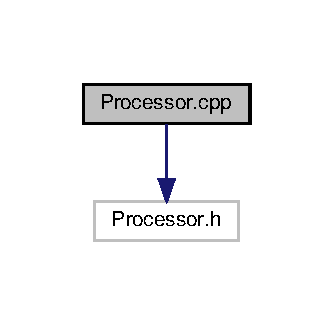
\includegraphics[width=160pt]{Processor_8cpp__incl}
\end{center}
\end{figure}

\hypertarget{processor_8h}{}\section{processor.\+h File Reference}
\label{processor_8h}\index{processor.\+h@{processor.\+h}}
This graph shows which files directly or indirectly include this file\+:\nopagebreak
\begin{figure}[H]
\begin{center}
\leavevmode
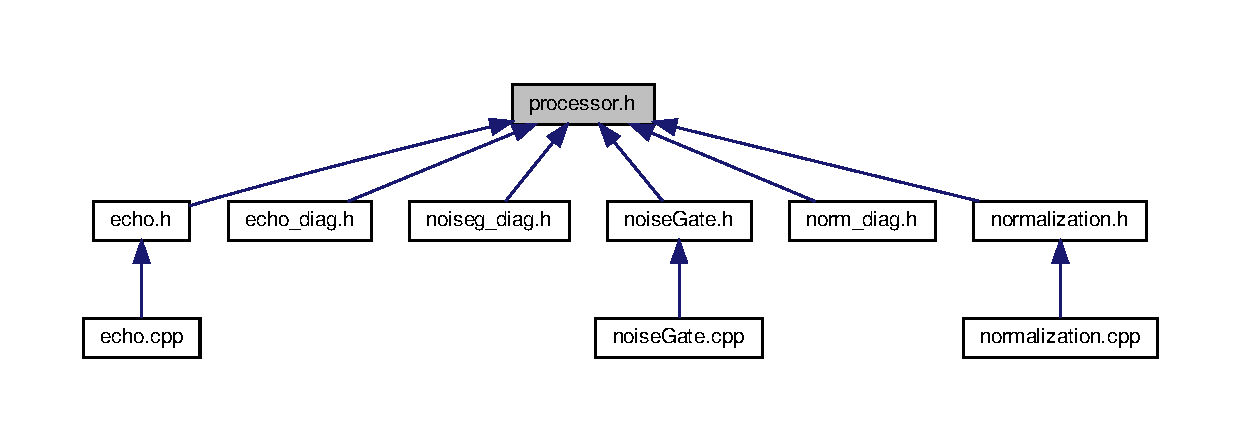
\includegraphics[width=350pt]{processor_8h__dep__incl}
\end{center}
\end{figure}
\subsection*{Classes}
\begin{DoxyCompactItemize}
\item 
class \hyperlink{classProcessor}{Processor}
\end{DoxyCompactItemize}

\hypertarget{README_8md}{}\section{R\+E\+A\+D\+M\+E.\+md File Reference}
\label{README_8md}\index{R\+E\+A\+D\+M\+E.\+md@{R\+E\+A\+D\+M\+E.\+md}}

\hypertarget{wav_8cpp}{}\section{wav.\+cpp File Reference}
\label{wav_8cpp}\index{wav.\+cpp@{wav.\+cpp}}
{\ttfamily \#include $<$iostream$>$}\newline
{\ttfamily \#include $<$string$>$}\newline
{\ttfamily \#include $<$fstream$>$}\newline
{\ttfamily \#include \char`\"{}wav.\+h\char`\"{}}\newline
Include dependency graph for wav.\+cpp\+:\nopagebreak
\begin{figure}[H]
\begin{center}
\leavevmode
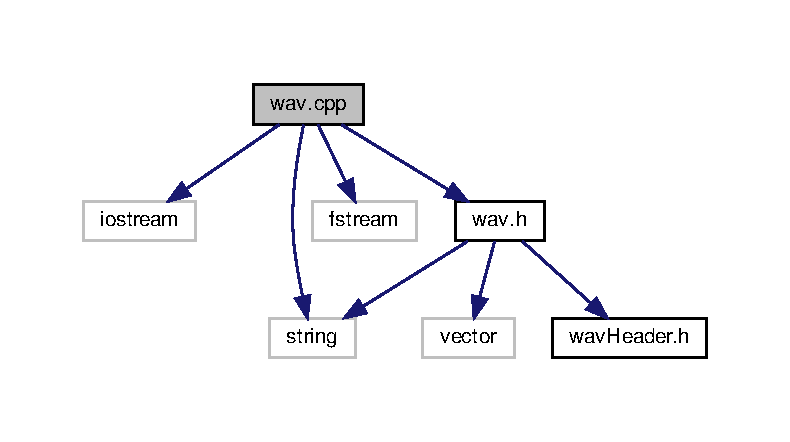
\includegraphics[width=350pt]{wav_8cpp__incl}
\end{center}
\end{figure}

\hypertarget{wav_8h}{}\section{wav.\+h File Reference}
\label{wav_8h}\index{wav.\+h@{wav.\+h}}
{\ttfamily \#include $<$string$>$}\newline
{\ttfamily \#include $<$vector$>$}\newline
{\ttfamily \#include \char`\"{}wav\+Header.\+h\char`\"{}}\newline
Include dependency graph for wav.\+h\+:\nopagebreak
\begin{figure}[H]
\begin{center}
\leavevmode
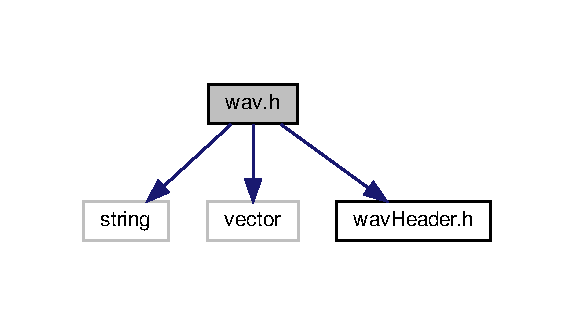
\includegraphics[width=276pt]{wav_8h__incl}
\end{center}
\end{figure}
This graph shows which files directly or indirectly include this file\+:\nopagebreak
\begin{figure}[H]
\begin{center}
\leavevmode
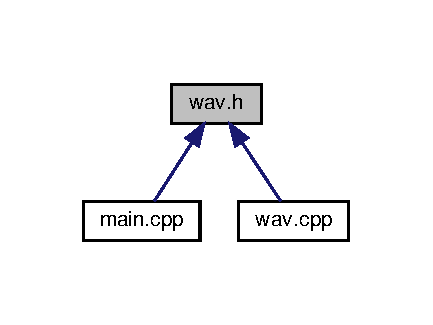
\includegraphics[width=208pt]{wav_8h__dep__incl}
\end{center}
\end{figure}
\subsection*{Classes}
\begin{DoxyCompactItemize}
\item 
class \hyperlink{classWav}{Wav}
\end{DoxyCompactItemize}

\hypertarget{Wave__Header_8h}{}\section{Wave\+\_\+\+Header.\+h File Reference}
\label{Wave__Header_8h}\index{Wave\+\_\+\+Header.\+h@{Wave\+\_\+\+Header.\+h}}
This graph shows which files directly or indirectly include this file\+:\nopagebreak
\begin{figure}[H]
\begin{center}
\leavevmode
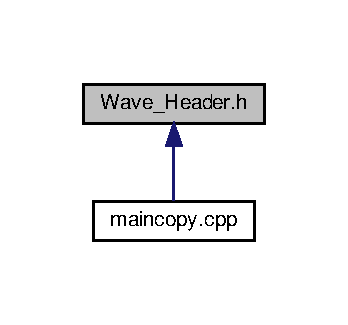
\includegraphics[width=167pt]{Wave__Header_8h__dep__incl}
\end{center}
\end{figure}
\subsection*{Classes}
\begin{DoxyCompactItemize}
\item 
struct \hyperlink{structWave__Header}{Wave\+\_\+\+Header}
\end{DoxyCompactItemize}
\subsection*{Typedefs}
\begin{DoxyCompactItemize}
\item 
typedef struct \hyperlink{structWave__Header}{Wave\+\_\+\+Header} \hyperlink{Wave__Header_8h_a7934a4bae79f1e47625eb97faef49be6}{Wave\+\_\+\+Header}
\end{DoxyCompactItemize}


\subsection{Typedef Documentation}
\mbox{\Hypertarget{Wave__Header_8h_a7934a4bae79f1e47625eb97faef49be6}\label{Wave__Header_8h_a7934a4bae79f1e47625eb97faef49be6}} 
\index{Wave\+\_\+\+Header.\+h@{Wave\+\_\+\+Header.\+h}!Wave\+\_\+\+Header@{Wave\+\_\+\+Header}}
\index{Wave\+\_\+\+Header@{Wave\+\_\+\+Header}!Wave\+\_\+\+Header.\+h@{Wave\+\_\+\+Header.\+h}}
\subsubsection{\texorpdfstring{Wave\+\_\+\+Header}{Wave\_Header}}
{\footnotesize\ttfamily typedef struct \hyperlink{structWave__Header}{Wave\+\_\+\+Header}  \hyperlink{structWave__Header}{Wave\+\_\+\+Header}}

This is a Wave Header struct 
\hypertarget{wavHeader_8h}{}\section{wav\+Header.\+h File Reference}
\label{wavHeader_8h}\index{wav\+Header.\+h@{wav\+Header.\+h}}
This graph shows which files directly or indirectly include this file\+:\nopagebreak
\begin{figure}[H]
\begin{center}
\leavevmode
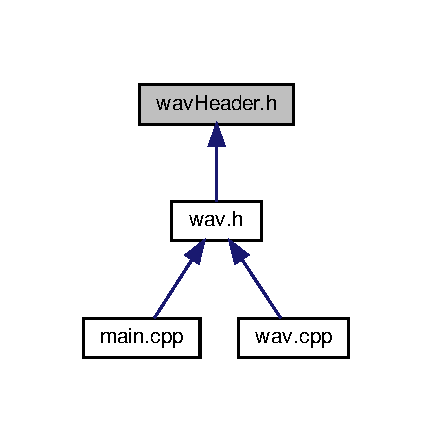
\includegraphics[width=208pt]{wavHeader_8h__dep__incl}
\end{center}
\end{figure}
\subsection*{Classes}
\begin{DoxyCompactItemize}
\item 
struct \hyperlink{structwavHeader}{wav\+Header}
\item 
struct \hyperlink{structdataChunk}{data\+Chunk}
\item 
struct \hyperlink{structFMT}{F\+MT}
\item 
struct \hyperlink{structSubChunkData}{Sub\+Chunk\+Data}
\end{DoxyCompactItemize}

%--- End generated contents ---

% Index
\backmatter
\newpage
\phantomsection
\clearemptydoublepage
\addcontentsline{toc}{chapter}{Index}
\printindex

\end{document}
